\chapter{Formal Concept Analysis}
\label{cha:form-conc-analys}

In this section we shall introduce almost all notions from the area of \emph{formal
  concept analysis}~\cite{fca-book} which are relevant for this work.  As a subfield of
order theory, formal concept analysis emerged as a distinctive discipline in the early
1980s as an attempt to restructure lattice theory~\cite{fca:Wille:1982}, and was back then
inspired by works of Birkhoff~\cite{books/math/Birkhoff67} and
Hentig~\cite{books/phil/Hentig72}.  Since then formal concept analysis has evolved into a
vivid theory with connections into knowledge representation, database theory and logic.

One of the main aspects of formal concept analysis we are interested in are the methods it
provides to extract \emph{implicational dependencies} from data.  To this end, we shall
discuss in detail the notions of \emph{implications} in formal contexts, \emph{bases} of
valid implications of formal contexts, and the computation of the \emph{canonical base} as
a particular example of a minimal base.  This will be done in
Sections~\ref{sec:bases-implications} and~\ref{sec:bases-implications}.  We shall also
discuss related topic like \emph{Galois connections} and \emph{closure operators}
(Section~\ref{sec:galois-connections}) and \emph{attribute exploration}
(Section~\ref{sec:attr-expl}.  Before we can do so, however, we have to introduce some of
the fundamental concepts of formal concept analysis such as \emph{formal contexts} and
\emph{contextual derivation}.  This will be done in Section~\ref{sec:form-cont-cont}.

Note that the introduction to formal concept analysis as given here is specifically
tailored towards the purpose of the whole work.  As such, the following exposition is not
complete in the sense that it discusses all the mathematical foundations of formal concept
analysis.  In particular, we may omit proofs or details of certain argumentations if they
are not relevant for our work.  In case more details are needed, we provide pointers to
the literature where those details can be found.

\section{Formal Contexts and Concept Lattices}
\label{sec:form-cont-cont}

We introduce the basic notions of formal concept analysis in this section.  Most
importantly, we shall discuss how formal concept analysis allows us to represent
complete lattices in terms of \emph{formal concept lattices} using the notion of
\emph{formal contexts}.

Let us briefly repeat the basic notions of order theory which are relevant for our further
considerations.  Let $P$ be a set and let ${\le} \subseteq P \times P$ be a binary
relation on $P$.  Then the pair $(P, \le)$ is called an \emph{(partially) ordered set} if
$\le$ is reflexive, transitive and antisymmetric.  Such structures can be visualize in
terms of \emph{order diagrams} (often called \emph{Hasse diagrams}) if they are finite
(and not too large).  For this way call two elements $x, y \in P$ with $x < y$
\emph{directly neighbored} in $(P, \le)$ if and only if there does not exist an element $z
\in P$ such that $x < z < y$.  Then to visualize $(P, \le)$ we mark for every element
$x \in P$ a node $v_x$ on the plane such that whenever $x < y$ it is true that the
ordinate (the second coordinate) of $v_x$ is strictly smaller then the one of $v_y$.
Then, we draw for every two elements $x, y$ with $x < y$ which are directly neighbored in
$(P, \le)$ an undirected line from $v_x$ to $v_y$.

Observe that this construction is not unique, and are many different possibilities (good
and bad) to visualize ordered sets in this way.  Also note that the naming $v_x$ of
vertices for elements $x$ is arbitrary and can be chosen as it suits.

\begin{Example}
  \label{expl:1}
  Let us consider the set $\set{1, 2, 3}$ with the usual order $\le$ on natural numbers.
  Then a line diagram of this order set is
  \begin{center}
    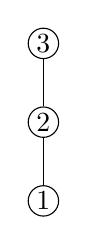
\begin{tikzpicture}[every node/.style = {draw, circle, inner sep = 1pt}]
      \node (A) {$3$};
      \node[below of=A] (B) {$2$};
      \node[below of=B] (C) {$1$};
      \draw (A) -- (B);
      \draw (B) -- (C);
    \end{tikzpicture}
  \end{center}
  We can readily read of this diagram that $1 < 2$ and $2 < 3$, because there are lines
  connecting the corresponding vertices.  But we can also see that $1 < 3$ because there
  is an \emph{ascending path} from $1$ to $3$.
\end{Example}

More generally, in a line diagram of an ordered set $(P, \le)$, two elements $x, y \in P$
satisfy $x \le y$ if and only if there is an ascending path from $x$ to $y$ in the line
diagram (where also paths of length 0 are allowed).

\begin{Example}
  \label{expl:2}
  Let $P = \set{ 1, 2, 3 }$ and consider the ordered set $(\subsets{\set{1,2,3}},
  \subseteq)$, where $\subsets{\set{1,2,3}}$ denotes the set of all subsets of
  $\set{1,2,3}$.  This set can be visualized as a line diagram as follows:
  \begin{center}
    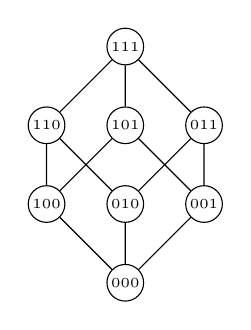
\begin{tikzpicture}[every node/.style = {draw, circle, inner sep = 1pt}]
      \node (0) at (0,0)  {\tiny 000};
      \node (1) at (-1,1) {\tiny 100};
      \node (2) at (0, 1) {\tiny 010};
      \node (3) at (1, 1) {\tiny 001};
      \node (4) at (-1,2) {\tiny 110};
      \node (5) at (0,2)  {\tiny 101};
      \node (6) at (1,2)  {\tiny 011};
      \node (7) at (0,3)  {\tiny 111};
      \draw{
        (0) -- (1)
        (0) -- (2)
        (0) -- (3)
        (1) -- (4)
        (1) -- (5)
        (2) -- (4)
        (2) -- (6)
        (3) -- (5)
        (3) -- (6)
        (4) -- (7)
        (5) -- (7)
        (6) -- (7)
      };
    \end{tikzpicture}
  \end{center}
  Here we denote subsets of $\set{1,2,3}$ by sequences of 0 and 1, meaning that if the
  first position is 1 if and only if the number 1 is an element of the corresponding
  subset, and so on.  Then 101 corresponds to the set $\set{1,3}$.
\end{Example}

An element $x \in P$ is said to be the \emph{smallest element} of $(P, \le)$ if and only
if $x \le y$ is true for all $y \in P$.  Likewise, $x$ is the \emph{greatest element} of
$(P, \le)$ if and only if $y \le x$ is true for all $y \in P$.  Note that neither smallest
nor greatest elements have to exist in $P$.  However, if these elements exist, they are
unique up to equivalence.

Let $Q \subseteq P$.  An element $x \in Q$ is said to be the \emph{smallest element} in
$Q$ (with respect to $(P, \le)$) if and only if $x \le y$ is true for all $y \in Q$;
\emph{greatest element} in $Q$ are defined likewise.  Again, neither smallest nor greatest
elements in $Q$ have to exist.

Let $x \in P$.  The \emph{order-ideal} ${\downarrow}x$ and the \emph{order-filter}
${\uparrow} x$ of $x$ in $(P, \le)$ are defined as
\begin{align*}
  {\downarrow} x &:= \set{ y \in P \mid y \le x },\\
  {\uparrow} x &:= \set{ y \in P \mid x \le y }.
\end{align*}
In other words, ${\downarrow} x$ contains all elements which are \emph{below} $x$ in $(P,
\le)$, and ${\uparrow} x$ contains all elements which are \emph{above} $x$ in $(P, \le)$.

Let again $Q \subseteq P$.  Then the sets ${\downarrow} Q$ and ${\uparrow} Q$ defined as
\begin{align*}
  {\uparrow} Q &:= \bigcap_{q \in Q} {\uparrow} q,\\
  {\downarrow} Q &:= \bigcap_{q \in Q} {\downarrow} q
\end{align*}
are called the set of \emph{upper bounds} and \emph{lower bounds} of $Q$ in $(P, \le)$,
respectively, where we employ the convention that $\bigcap \emptyset = P$.  If ${\uparrow}
Q$ has a smallest element (a \emph{least upper bound}) in $(P, \le)$, it is called the
\emph{supremum} of $Q$ in $(P, \le)$ and is denoted by $\sup Q$.  Likewise, if
${\downarrow} Q$ has a greatest element (a \emph{greatest lower bound}) in $(P, \le)$,
then it is called the \emph{infimum} of $Q$ in $(P, \le)$ and is denoted by $\inf Q$.

Note again that neither infimum nor supremum have to exist in $(P, \le)$.

\begin{Example}
  \label{expl:3}
  Let $P = \set{ a, b, c }$ and let $\le$ be given by the smallest order relation that
  satisfies $a < b$ and $a < c$.  Then $\inf\set{b,c}$ exists in $(P, \le)$ and is equal
  to $a$.  However, $\sup\set{b, c}$ does not exist in $(P, \le)$, as ${\uparrow} b \cap
  {\uparrow} c = \emptyset$.
\end{Example}

\noindent%
Structures in which supremum and infimum always exist for \emph{finite} sets $Q$ are
called \emph{lattices}.  If the sets $Q$ can be chosen arbitrary, then we call such a
structure a \emph{complete lattice}.

\begin{Definition}[Lattice]
  \label{def:lattice}
  Let $\alg L = (L, \le)$ be an ordered set.  Then $\alg L$ is called a \emph{lattice} if
  and only if for each finite $Q \subseteq L$ there exist both $\sup Q$ and $\inf Q$ in
  $\alg L$.  If for all $Q \subseteq L$ there exist both $\sup Q$ and $\inf Q$ in $\alg
  L$, then $\alg L$ is called a \emph{complete lattice}.
\end{Definition}

\noindent%
From time to time we may also use another notation for $\inf$ and $\sup$: if $Q$ is
finite, then $Q = \set{ q_1, \dots, q_n }$ and we may write
\begin{align*}
  q_1 \wedge \dots \wedge q_n &\quad\text{instead of}\quad \inf Q,\\
  q_1 \vee \dots \vee q_n &\quad\text{instead of}\quad \sup Q.
\end{align*}
If $Q$ is infinite, then the notation
\begin{align*}
  \bigwedge Q &\quad\text{instead of}\quad \inf Q,\\
  \bigvee Q &\quad\text{instead of}\quad \sup Q
\end{align*}
is rather common.

Note that every finite lattice is also a complete lattice.  Moreover, every complete
lattice has a smallest and greatest element, given by $\sup\emptyset$ and $\inf\emptyset$,
respectively.  Furthermore, every ordered set $(P, \le)$ in which the supremum exists for
each $Q \subseteq P$ is already a complete lattice, as the infimum is then given by
\begin{equation*}
  \inf Q = \sup\set{ x \in P \mid \forall y \in Q \holds x \le y }.
\end{equation*}
The same is of course true if supremum and infimum are exchanged.

The ordered sets from Examples~\ref{expl:1} and~\ref{expl:2} are lattices, but not the one
from~\ref{expl:3}.  More generally, if $P$ is a set, then $(\subsets{P}, \subseteq)$ is
always a complete lattice.

The study of lattices as mathematical structures has received much interest over the last
decades and thus constitutes a major branch of order
theory~\cite{Gratzer,books/math/Davey02,books/math/Birkhoff67}.  Additionally, (complete)
lattices also allow for a quite natural interpretation as a hierarchy of
\emph{generalizations} and \emph{specializations}: an element $x$ is below an element $y$
if and only if $x$ is more \emph{special} than $y$, or alternatively, if $y$ is more
\emph{general} than $x$.  Then for a set $Q$ of elements its supremum $\sup Q$ can be
thought of as a \emph{most-specific generalization} of all elements in $Q$, and $\inf Q$
can be seen likewise as the most \emph{general specialization} of all elements in $Q$.

Formal concept analysis now provides an approach to understand complete lattice in terms
of this interpretation, by representing these lattices in terms of \emph{objects} and
their \emph{attributes}.  For this, we need to introduce the notion of a \emph{formal
  context}.

\begin{Definition}[Formal Context]
  \label{def:formal-context}
  A \emph{formal context} $\con K$ is constituted of three sets $G, M, I$, where $I
  \subseteq G \times M$.  Most often, we shall identify $\con K$ with the triple $(G, M,
  I)$, \ie $\con K = (G, M, I)$.  We shall call $G$ the set of \emph{objects} of $\con K$,
  $M$ the set of \emph{attributes} of $\con K$ and $I$ the \emph{incidence} of $\con K$.
  Two formal contexts are equal if and only if their sets of objects, attributes and their
  incidences are equal, respectively.
\end{Definition}

Formal contexts can be thought of as simple data structures which record for a set of
objects the set of attributes those objects have.  More precisely, we shall say that in a
formal context $\con K$ an object $g \in G$ \emph{has} an attribute $m$ if and only if
$(g, m) \in I$.

\begin{Example}
  \label{expl:star-trek}
  Let us consider a small toy example $\con K_{\mathsf{TNG}}$ to illustrate the definition
  of a formal context.  As sets of objects we choose some fictional characters from
  \emph{Star Trek: The Next Generation}, namely
  \begin{equation*}
    G := \set{ \mathsf{Picard}, \mathsf{Worf}, \mathsf{Data}, \mathsf{BorgQueen} }.
  \end{equation*}
  As sets of attributes we choose
  \begin{equation*}
    M := \set{ \mathsf{Human}, \mathsf{Honorable}, \mathsf{Artificial}, \mathsf{Star
        Fleet} }.
  \end{equation*}
  To illustrate the incidence relation of our examples formal context we make use of a
  \emph{cross table}, \ie we depict $\con K_{\mathsf{TNG}}$ as a table where the rows are
  labeled with objects and the columns are labeled with attributes.  Then in every cell we
  write a cross if and only if the objects labeling the corresponding row has the
  attribute labeling the corresponding column.
  \begin{equation*}
    \def\x{\times}
    \begin{array}{r|*{4}{c}}
      \toprule
      \con K_{\mathsf{TNG}} & \mathsf{Human} & \mathsf{Honorable} & \mathsf{Artificial} & \mathsf{Star Fleet} \\
      \midrule
      \mathsf{Picard} & \x & \x & & \x \\
      \mathsf{Worf} & & \x & & \x \\
      \mathsf{Data} & & \x & \x & \x \\
      \mathsf{BorgQueen} & & & \x & \\
      \bottomrule
    \end{array}
  \end{equation*}
  Then \textsf{BorgQueen} has the attribute \textsf{Artificial}, but not \textsf{Honorable}.
\end{Example}

To now expose the connection between formal contexts on the one hand and complete lattices
on the other we shall introduce the \emph{derivation operators} in formal contexts.

\begin{Definition}[Contextual Derivation]
  \label{def:contextual-derivation}
  Let $\con K = (G, M, I)$ be a formal context and let $A \subseteq G$ be a set of
  objects.  Then the set of \emph{common attributes} $A'$ of $A$ is defined to be
  \begin{equation*}
    A' := \set{ m \in M \mid \forall g \in G \holds (g, m) \in I }.
  \end{equation*}
  Likewise, for a set $B \subseteq M$ of attributes we define the set $B'$ of \emph{shared
    objects} as
  \begin{equation*}
    B' := \set{ g \in G \mid \forall m \in M \holds (g, m) \in I }.
  \end{equation*}
  The functions $A \mapsto A'$ and $B \mapsto B'$ are called the \emph{derivation
    operators} of $\con K$, and the sets $A'$ and $B'$ are called the \emph{derivations}
  of $A$ and $B$ in $\con K$, respectively.
\end{Definition}

For $(A')'$ we may also simply write $A''$.

Note that both derivation operators are denoted by $(\cdot)'$, which usually does not lead
to confusion, as it is most often clear from the context whether we deal with a set of
objects or a set of attributes from which we want to compute its derivation.  If it
nevertheless happens that a single name for the derivation operator leads to confusion,
then we shall locally introduce separate names for both of them.

What occurs more often, for example in Chapters~\ref{cha:expl-conf}
and~\ref{cha:model-expl-conf}, is the derivation of sets in \emph{different contexts}.
For example we may have given two formal contexts $\con K_1 = (G_1, M_1, I_1)$ and $\con
K_2 = (G_2, M_2, I_2)$ and a set $A \subseteq M_1 \cap M_2$.  Then when writing $A'$ it is
not clear in which context we do the derivation.  To remedy this, we shall add a subscript
to the set $A$ to make clear of which context we consider it as a set of attributes:
$A_{\con K_1}$ denotes the set $A$ considered as a set of attributes in $\con K_1$, and
likewise $A_{\con K_2}$.  While this notation is not useful as it stands, it becomes handy
if we consider derivations of $A$: $(A_{\con K_1})'$ denotes the derivation of $A$ in the
formal context $\con K_1$, while $(A_{\con K_2})'$ does the same for the formal context
$\con K_2$.  Of course, we can drop the parentheses if they do not lead to ambiguity and
write $A_{\con K_1}'$ and $A_{\con K_2}'$ instead.  Of course, the same can be done for
sets of objects.  In particular, instead of writing $(A_{\con K_1}')_{\con K_1}'$ we shall
often only write $A_{\con K_1}''$.

\begin{Example}
  \label{expl:4}
  Consider our Star Trek example context from~\ref{expl:star-trek} and let $A :=
  \set{\mathsf{Human}}$.  Then $A' = \set{ \mathsf{Picard} }$, $A'' = \set{
    \mathsf{Human}, \mathsf{Honorable}, \mathsf{Star Fleet} }$, and $A''' = \set{
    \mathsf{Picard} } = A'$.
\end{Example}

The case that $A''' = A'$ is true in the previous example is not a coincidence, but rather
an instance of a more general result: the derivation operators of a formal context form a
\emph{Galois connection} between the ordered sets $(\subsets{G}, \subseteq)$ and
$(\subsets{M}, \subseteq)$.

\begin{Lemma}
  \label{lem:derivation-is-galois-connection}
  Let $\con K = (G, M, I)$ be a formal context and let $A \subseteq M$ and $B \subseteq
  G$.  Then it is true that
  \begin{equation}
    \label{eq:1}
    A \subseteq B' \iff B \subseteq A'.
  \end{equation}
  From this the following properties of the derivation operators of $\con K$ can be
  derived: let $A, A_1, A_2 \subseteq M$ and $B, B_1, B_2 \subseteq G$.  Then
  \begin{enumerate}[i. ]
  \item $A_1 \subseteq A_2 \implies A_2' \subseteq A_1'$,
  \item $B_1 \subseteq B_2 \implies B_2' \subseteq B_1'$,
  \item $A \subseteq A''$,
  \item $B \subseteq B''$,
  \item $A' = A'''$,
  \item $B' = B'''$.
  \end{enumerate}
\end{Lemma}
%
In the proof of the lemma we shall only show Equation~\eqref{eq:1}, as the remaining
claims are a then an immediate consequence of the more general result
Lemma~\ref{lem:properties-of-galois-connections} on Galois connections.
%
\begin{Proof}[\thref{lem:derivation-is-galois-connection}]
  We can easily compute that
  \begin{align*}
    A \subseteq B'
    & \iff \forall m \in A \holds m \in B' \\
    & \iff \forall m \in A \;\forall g \in B \holds (g,m) \in I \\
    & \iff \forall g \in B \;\forall m \in A \holds (g,m) \in I \\
    & \iff \forall g \in B \holds g \in A' \\
    & \iff B \subseteq A'
  \end{align*}
  which shows the claim.
\end{Proof}

Another useful property of the derivation operators is
\begin{equation*}
  A' = \bigcap_{a \in A} \set{a}'
\end{equation*}
for $A \subseteq M$.  This can easily be generalized into the following statement.

\begin{Lemma}
  \label{lem:piecewise-derivation}
  Let $\con K = (G, M, I)$ be a formal context, let $A \subseteq M$ and let $(B_j \mid j
  \in J)$ be a family of sets $B_j \subseteq M$ such that
  \begin{equation*}
    A = \bigcup_{j \in J} B_j.
  \end{equation*}
  Then
  \begin{equation}
    \label{eq:2}
    A' = \bigcap \set{ B_j' \mid j \in J }.
  \end{equation}
  In particular, for every $\mathcal{A} \subseteq \subsets{M}$ it is true that
  \begin{equation}
    \label{eq:3}
    \bigcap_{A \in \mathcal{A}} A' = \bigl(\bigcup_{A \in \mathcal{A}} A'\bigr).
  \end{equation}
\end{Lemma}
%
Of course, the same is true if $A$ and all $B_j$ are sets of objects instead of sets of
attributes.
%
\begin{Proof}[\thref{lem:piecewise-derivation}]
  Since $B_j \subseteq A$ for all $j \in J$, we can infer from
  \thref{lem:derivation-is-galois-connection} that $A' \subseteq B_j'$.  It therefore
  suffices to show that $A' \supseteq \bigcap \set{ B_j' \mid j \in J }$.

  To this end, let $g \in \bigcap \set{ B_j' \mid j \in J }$.  Then $g \in B_j'$ for each
  $j \in J$, and therefore $\set{g}' \supseteq B_j$, again for all $j \in J$.  Since $A =
  \bigcup_{j \in J} B_j$, we obtain from this that $\set{g}' \supseteq A$, and thus $g \in
  A'$, as required.
\end{Proof}

We have claimed earlier that there exists a close connection between complete lattices on
the one hand and formal contexts on the other.  Having introduced the derivation
operators, we are now able to expose this connection.  To this end, we shall introduce the
notion of \emph{formal concepts} of a formal context.

\begin{Definition}[Formal Concept]
  \label{def:formal-concept}
  Let $\con K = (G, M, I)$ be a formal context.  Then a \emph{formal concept} of $\con K$
  is a pair $(A, B)$ such that $A \subseteq G, B \subseteq M$, and $A' = B, B' = A$ holds.
  The first entry of a formal concept is called its \emph{extent}, and the second one
  called its \emph{intent}.  The set of all formal concepts of $\con K$ is denoted by
  $\BV(\con K)$, the set of all extents of (formal concepts of) $\con K$ is denoted by
  $\Ext\con K$, and the set of all intents of (formal concepts of) $\con K$ is denoted by
  $\Int\con K$.
\end{Definition}

Note that for each $A \subseteq M$, the pair $(A, A')$ is a formal concept of $\con K$.
Moreover, a set $A \subseteq M$ is an intent of $\con K$ if and only if $A = A''$: if $A =
A''$, then $(A'', A')$ is a formal concept of $\con K$, and if $(A, B)$ is a formal
concept of $\con K$, then $A'' = B' = A$.  The same is of course true for $B \subseteq G$:
$B$ is an extent of $\con K$ if and only if $B = B''$.

Formal concepts have a strong philosophical motivation, as they are an attempt to
formalize the rather vague notion of a \emph{concept}.  This formalization is based on the
perception that every formal concept is uniquely determined by the objects which are
instances of it, its \emph{extension}, as well as by a characterization in terms of
attributes, its \emph{intension}.  We shall, however, not pursue this philosophical
motivation any further here, as it is not immediately relevant for our work.
See~\cite{fca-book} for further discussion and references.

\begin{Example}
  \label{expl:5}
  Two formal concepts of $\con K_{\mathsf{TNG}}$ from Example~\ref{expl:star-trek} are
  \begin{gather*}
    (\set{\mathsf{Picard}}, \set{\mathsf{Human}, \mathsf{Honorable},
      \mathsf{StarFleet}}),\\
    (\set{\mathsf{Picard}, \mathsf{Worf}, \mathsf{Data}}, \set{\mathsf{Honorable}}).
  \end{gather*}
  The first formal concept could be said to represent the concept of an \emph{honorable
    human}, which in $\con K_{\mathsf{TNG}}$ has \textsf{Picard} as its only instance.
  The second formal concept describes everything \emph{honorable}, having as extension
  \textsf{Picard}, \textsf{Worf} and \textsf{Data}.
\end{Example}

Formal concepts can be ordered by \emph{generality}: a formal concept $(A_1, B_1)$ is
\emph{more general} than another formal concept $(A_2, B_2)$ if it covers more objects,
\ie if
\begin{equation*}
  A_1 \subseteq A_2.
\end{equation*}

\begin{Definition}[Concept Lattice]
  \label{def:concept-lattice}
  Let $\con K = (G, M, I)$ be a formal context.  We define the relation $\le$ on $\BV(\con
  K)$ by
  \begin{equation*}
    (A_1, B_1) \leq (A_2, B_2) \diff A_1 \subseteq A_2.
  \end{equation*}
  The structure $\alg{\BV}(\con K) := (\BV(\con K), \leq)$ is called the \emph{concept
    lattice} of $\con K$.
\end{Definition}

By \thref{lem:derivation-is-galois-connection} we can observe that
\begin{equation*}
  (A_1, B_1) \leq (A_2, B_2) \iff B_2 \subseteq B_1,
\end{equation*}
as $B_1 = A_1'$ and $B_2 = A_2'$.  Furthermore, it is rather easy to see that the relation
$\leq$ from \thref{def:concept-lattice} is an order relation on $\BV(\con K)$.  However,
even more is true, namely that $\alg{\BV}(\con K)$ is indeed a complete lattice.

\begin{Theorem}
  \label{thm:concept-lattices-are-complete-lattices}
  Let $\con K$ be a formal context.  Then $\alg{\BV}(\con K)$ is a complete lattice, and
  for formal concepts $((A_j, B_j) \mid j \in J)$ of $\con K$ we have
  \begin{align*}
    \sup \set{ (A_j, B_j) \mid j \in J } = \Bigl( \bigl( \bigcap_{j \in J} B_j \bigr)' ,
    \bigcap_{j \in J} B_j \Bigr), \\
    \inf \set{ (A_j, B_j) \mid j \in J } = \Bigl( \bigcap_{j \in J} A_j, \bigl( \bigcap_{j
      \in J} A_j \bigr)' \Bigr).
  \end{align*}
\end{Theorem}

On the other hand, every complete lattice can be represented as a concept lattice of a
suitably chosen formal context.  To formalize this correctly, we shall introduce the
notion of an \emph{order isomorphism} between two ordered sets.

\begin{Definition}[Order Isomorphism]
  \label{def:order-isomorphism}
  Let $\alg P = (P, \leq_1)$ and $\alg Q = (Q, \leq_2)$ be two ordered sets.  A bijective
  mapping $\phi \colon P \to Q$ is called an \emph{order isomorphism} if and only if
  $\phi$ is \emph{order-preserving} and \emph{order-reflecting}, \ie it is true for all
  $a, b \in P$ that
  \begin{equation*}
    a \leq_1 b \iff \phi(a) \leq_2 \phi(b).
  \end{equation*}
\end{Definition}

The statement now is that every for complete lattice is \emph{order-isomorphic} to some
concept lattice.

\begin{Theorem}
  \label{thm:complete-lattices-are-concept-lattices}
  Let $\alg V = (V, \leq_V)$ be a complete lattice.  Then the mapping $\phi \colon V \to
  \BV(\con K)$ defined by
  \begin{equation*}
    \phi(v) := (\set{ w \in V \mid w \leq_V v}, \set{ w \in V \mid v \leq_V w })
  \end{equation*}
  is an order isomorphism between $\alg V$ and $\alg{\BV}(V, V, \leq_V)$.
\end{Theorem}

Both \thref{thm:concept-lattices-are-complete-lattices} and
\thref{thm:complete-lattices-are-concept-lattices} are actually part of the Basic Theorem
of formal concept analysis~\cite[Theorem 3]{fca-book}.  We shall not give a proof of it
here, as it is not within the scope of this work.

\begin{Example}
  \label{expl:star-trek-concept-lattice}
  Let us consider the formal context $\con K_{\mathsf{TNG}}$ of
  Example~\ref{expl:star-trek} a last time, and let us draw the concept lattice of $\con
  K_{\mathsf{TNG}}$ in form of a line diagram.  There are 6 formal concepts of $\con
  K_{\mathsf{TNG}}$, and they can depicted as shown in
  Figure~\ref{fig:star-trek-concept-lattice}.

  \begin{figure}[tp]
    \centering
    \begin{tikzpicture}[scale=2, every node/.style = { draw, circle }]
      \node (1) at (0,0) {};
      \node (2) at (-1,1) {};
      \node (3) at (1,1) {};
      \node (4) at (0,2) {};
      \node (5) at (2,2) {};
      \node (6) at (1,3) {};
      \draw {
        (1) -- (2)
        (1) -- (3)
        (2) -- (4)
        (3) -- (4)
        (3) -- (5)
        (4) -- (6)
        (5) -- (6)
      };
      \begin{scope}[every node/.style = { draw=none, inner sep=1pt, fill=white },
         node distance = 0.2cm and 0.2cm]
        \node[above=of 2] {\small\textsf{Human}};
        \node[below=of 2] {\small\textsf{Picard}};
        \node[below=of 3] {\small\textsf{Data}};
        \node[below=of 4] {\small\textsf{Worf}};
        \node[above=of 4] {\small\textsf{StarFleet}, \textsf{Honorable}};
        \node[below=of 5] {\small\textsf{BorgQueen}};
        \node[above=of 5] {\small\textsf{Artificial}};
      \end{scope}
    \end{tikzpicture}
    \caption{Drawing of the concept lattice of $\con K_{\mathsf{TNG}}$}
    \label{fig:star-trek-concept-lattice}
  \end{figure}

  The line diagram of Figure~\ref{fig:star-trek-concept-lattice} uses an abridged
  annotation which is common for concept lattices: instead of annotating every node in the
  diagram with the formal concept it represents (which would yield an unreadable diagram),
  we only write every object $g$ of $\con K_{\mathsf{TNG}}$ below the \emph{smallest}
  formal concept that has $g$ in its extent.  This formal concept always exists by
  \thref{thm:concept-lattices-are-complete-lattices}.  Then, by the definition of the
  order on formal concepts, every formal concept which can be reached from the one labeled
  with $g$ by an \emph{ascending} path in the line diagram has $g$ in its diagram, and all
  other formal concepts have $g$ not in their extent.  For example, the formal concept
  labeled with \textsf{Picard} has this object in its intent, as well as the two formal
  concepts above it.  No other formal concept has \textsf{Picard} in its intent.

  Likewise, for we write every attribute $m$ of $\con K_{\mathsf{TNG}}$ only at the
  \emph{largest} formal concept that has this attribute in its intent.  Then every formal
  concept that can be reached from the one labeled with $m$ by a \textsf{descending} path
  in the line diagram has $m$ in its intent, and all the others have not.  Therefore, the
  node labeled with \textsf{Artificial} has this attribute in its intent, as has the
  formal concept labeled with \textsf{Data} and the bottom concept.  No other formal
  concept has \textsf{Artificial} in its intent.
\end{Example}

\section{Galois Connections and Closure Operators}
\label{sec:galois-connections}

For the proof of \thref{lem:derivation-is-galois-connection} we invoked some general
arguments from the theory of Galois connections between ordered sets.  The notion of a
Galois connection is fundamental for order theory, and is closely connected to other
important concepts such as closure operators.  As both Galois connections and closure
operators play an important role in this work, we shall review their general theory in
this section, to the extent needed in this work.

\begin{Definition}[Galois Connection]
  \label{def:galois-connection}
  Let $\alg P = (P, \leq_P), \alg Q = (Q, \leq_Q)$ be two ordered sets, and let $\phi
  \colon P \to Q$ and $\psi \colon Q \to P$ be two mappings.  Then the tuple $(\alg P,
  \alg Q, \phi, \psi)$ is called a \emph{Galois connection} between $\alg P$ and $\alg Q$
  if and only if
  \begin{equation}
    \label{eq:4}
    x \leq_P \psi(y) \iff y \leq_Q \phi(x)
  \end{equation}
  is true for all $x \in P$, $y \in Q$.
\end{Definition}

Note that this form of a Galois connection is sometimes called an \emph{antitone} Galois
connection, as the position of the elements $x$ and $y$ is reversed.  There is the
corresponding notion of an \emph{isotone} Galois connection, where Equation~\eqref{eq:4}
is replaced by
\begin{equation}
  \label{eq:5}
  x \leq_P \psi(y) \iff \phi(x) \leq_Q y.
\end{equation}
Of course, both notions are closely related: if we denote with $\alg Q^d = (Q,
\leq_Q^{-1})$ the \emph{dual} of the ordered set $\alg Q$, then $(\alg P, \alg Q, \phi,
\psi)$ is an antitone Galois connection if and only if $(\alg P, \alg Q^d, \phi, \psi)$ is
an isotone Galois connection.

\begin{Example}
  \begin{enumerate}[i. ]
  \item If $\phi$ is an order isomorphism from $\alg P = (P, \leq_P)$ to $\alg Q = (Q,
    \leq_Q)$, then $(\alg P, \alg Q, \phi, \phi^{-1})$ is an isotone Galois connection,
    because
    \begin{align*}
      x \leq_P \phi^{-1}(y)
      &\iff \phi(x) \leq_Q \phi(\phi^{-1}(y))\\
      &\iff \phi(x) \leq_Q y
    \end{align*}
    is true for all $x \in P$ and $y \in Q$.

    On the other hand, if $\phi \colon P \to Q$ is a bijective mapping such that $(\alg P,
    \alg Q, \phi, \phi^{-1})$ is an isotone Galois connection, then clearly $\phi$ is an
    order isomorphism by \thref{lem:properties-of-galois-connections}.  In this sense are
    Galois connections a generalization of order isomorphism.
  \item If $\con K = (G, M, I)$ is a formal context, then the derivation operators
    $(\cdot)' \colon \subsets{G} \to \subsets{M}$ and $(\cdot)' \colon \subsets{M} \to
    \subsets{G}$ form an antitone Galois connection by
    \thref{lem:derivation-is-galois-connection}.
  \end{enumerate}
\end{Example}

Indeed, the converse of the last example is also true to some extent, \ie every antitone
Galois connection between powerset lattices $(\subsets{G}, \subseteq), (\subsets{M},
\subseteq)$ can be represented by a formal context $\con K$, such that the derivation
operators of $\con K$ are just the mappings from the Galois connections.  However, we
shall not go into details here, as this is not relevant for the purpose of our work.
See~\cite{fca-book} for more details.

Instead, we shall review some useful properties of antitone Galois connections.

\begin{Lemma}
  \label{lem:properties-of-galois-connections}
  Let $(\alg P, \alg Q, \phi, \psi)$ be an antitone Galois connection between the ordered
  sets $\alg P = (P, {\leq_P})$ and $\alg Q = (Q, \leq_Q)$.  Then the following statements
  hold for all $a_1, a_2 \in P$ and $b_1, b_2 \in Q$:
  \begin{enumerate}[i. ]
  \item\label{item:1} $a_1 \leq_P a_2 \implies \phi(a_2) \leq_Q \phi(a_1)$,
  \item\label{item:2} $b_1 \leq_Q b_2 \implies \psi(b_2) \leq_P \phi(b_1)$,
  \item\label{item:3} $a_1 \leq_P \psi(\phi(a_1))$,
  \item\label{item:4} $b_1 \leq_Q \phi(\psi(b_1))$,
  \item\label{item:5} $\phi(a_1) = \phi(\psi(\phi(a_1)))$,
  \item\label{item:6} $\psi(b_1) = \psi(\phi(\psi(b_1)))$.
  \end{enumerate}
\end{Lemma}
\begin{Proof}
  We only show statements~\ref{item:1}, \ref{item:3} and~\ref{item:5}, as the others
  follow similar arguments.

  We immediately obtain the truth of~\ref{item:3}, since from $\phi(a_1) \leq_Q \phi(a_1)$
  we can infer $a_1 \leq_Q \psi(\phi(a_1))$ by definition~\eqref{eq:4} of a Galois
  connection.

  Then for~\ref{item:1} we assume $a_1 \leq_P a_2$ and now by~\ref{item:3} that then $a_1
  \leq_P \psi(\phi(a_2))$.  Using again the definition of a Galois connection we obtain
  that $\phi(a_2) \leq_Q \phi(a_1)$.

  Finally, for~\ref{item:5} we already know that $\phi(\psi(\phi(a_1))) \leq_Q \phi(a_1)$
  is true.  On the other hand, $\psi(\phi(a_1)) \leq_Q \psi(\phi(a_1))$, so by the
  definition of a Galois connection, we obtain $\phi(a_1) \leq_P \phi(\psi(\phi(a_1)))$.
  Since $\leq_P$ is antisymmetric, equality follows.
\end{Proof}

Galois connections are closely related to the notion of \emph{closure operators}.

\begin{Definition}[Closure Operator]
  \label{def:closure-operator}
  Let $\alg P = (P, \leq_P)$ be an ordered set, and let $c \colon P \to P$ be a mapping.
  Then $c$ is called a \emph{closure operator} on $\alg P$ if and only if
  \begin{enumerate}[i. ]
  \item $a \leq_P c(a)$ for all $a \in P$ ($c$ is \emph{extensive}),
  \item $a \leq_P b \implies c(a) \leq_P c(b)$ for all $a, b \in P$ ($c$ is
    \emph{monotone}), and
  \item $c(a) = c(c(a))$ for all $a \in P$ ($c$ is \emph{idempotent}).
  \end{enumerate}
  A set of the form $c(a)$ for $a \in P$ is called the  \emph{closure} of $a$ under $c$.
  An element $a \in P$ is called \emph{closed} under $c$ if and only if $a = c(a)$.
\end{Definition}

Closure operators arise naturally in many situations, and we shall encounter them in the
next section when we introduce implication.  Moreover, closure operators and Galois
connections always appear together: If $(\alg P, \alg Q, \phi, \psi)$ is a Galois
connection, then the mapping $\psi \circ \phi$ is a closure operator on $\alg P$, and the
mapping $\phi \circ \psi$ is a closure operator on $\alg Q$.  This is true because we know
that $\psi \circ \phi$ is extensive
(\ref{lem:properties-of-galois-connections},~\ref{item:3}), monotone
(\ref{lem:properties-of-galois-connections},~\ref{item:1} and~\ref{item:2}) and idempotent
(\ref{lem:properties-of-galois-connections},~\ref{item:5}), \ie a closure operator.
Showing that $\phi \circ \psi$ is a closure operator as well can be done similarly.

Conversely, if $c$ is a closure operator on the ordered set $\alg P$, then there always
exists a Galois connection $(\alg P, \alg Q, \phi, \psi)$ such that $c = \psi \circ \phi$.
However, we shall not go into details here, as this is not necessary for our work.
See~\cite{fca-book} for more details on this.

There are two interesting properties of closure operators which are also relevant for our
purpose here, and which we shall therefore discuss here.  The first observation is that if
$c$ is a closure operator on the ordered set $\alg P$, that then the infimum $c(x) \wedge
c(y)$ is again closed for all $x, y \in P$.  This is because on the one hand we have
\begin{align*}
  c(c(x) \wedge c(y)) &\leq_P c(c(x)) = c(x),\\
  c(c(x) \wedge c(y)) &\leq_P c(c(y)) = c(y),
\end{align*}
by monotonicity and idempotency of $c$.  Therefore $c(c(x) \wedge c(y)) \leq_P c(x) \wedge
c(y)$.  On the other hand, $c(x) \wedge c(y) \leq_P c(c(x) \wedge c(y))$ because $c$ is
extensive, and therefore
\begin{equation}
  \label{eq:13}
  c(c(x) \wedge c(y)) = c(x) \wedge c(y),
\end{equation}
and therefore $c(x) \wedge c(y)$ is closed.  It is also not hard to see that this
argumentation can be lifted to arbitrary infima, \ie for all $Q \subseteq P$, the element
\begin{equation*}
  \bigwedge_{x \in Q} c(x)
\end{equation*}
is closed under $c$.  In other words, the closed sets of $c$ always form a complete
sublattice of $\alg P$.

In particular, for all $x \in P$ there always exists a smallest element $z \in P$ above
$x$ which is closed under $c$, namely
\begin{equation*}
  z = \bigwedge_{y \in P, x \leq_P c(y)} c(y) = c(x).
\end{equation*}

\section{Implications}
\label{sec:implications-sets}

Let us recall Example~\ref{expl:star-trek}, were we had considered the formal context
$\con K_{\mathsf{TNG}}$ with
\begin{equation*}
  \def\x{\times}
  \begin{array}{r|*{4}{c}}
    \toprule
    \con K_{\mathsf{TNG}} & \mathsf{Human} & \mathsf{Honorable} & \mathsf{Artificial} & \mathsf{StarFleet} \\
    \midrule
    \mathsf{Picard} & \x & \x & & \x \\
    \mathsf{Worf} & & \x & & \x \\
    \mathsf{Data} & & \x & \x & \x \\
    \mathsf{BorgQueen} & & & \x & \\
    \bottomrule
  \end{array}
\end{equation*}
In this formal context we see that whenever an object has the attribute
\textsf{StarFleet}, it also has the attribute \textsf{Honorable}.  This expresses a
certain dependency between these two attributes, in the sense that \textsf{StarFleet}
\emph{implies} \textsf{Honorable} in the formal context $\con K_{\mathsf{TNG}}$.  Knowing
such \emph{implicational dependencies} between attributes in a formal context can be very
helpful, for example for reducing databases by transferring them into suitable normal
forms or, as in our case, for learning knowledge from data.

We will model such implicational dependencies by means of \emph{implications} on sets,
which may be \emph{valid} in a formal context.

\begin{Definition}[Implications, Validity in Formal Contexts]
  Let $M$ be a set.  Then an implication $A \to B$ on $M$ is constituted of two sets $A, B
  \subseteq M$, where $A$ is called the \emph{premise} of $A \to B$, and $B$ is called the
  \emph{conclusion} of $A \to B$.  The set of all implications on $M$ is denoted by
  $\Imp(M)$.

  Let $\con K = (G, M, I)$ be a formal context.  An implication $(A \to B) \in \Imp(M)$ is
  said to be \emph{valid} in $\con K$ (or: \emph{holds} in $\con K$) if and only if $A'
  \subseteq B'$.  We shall write $\con K \models (A \to B)$ in this case, and $\con K
  \models \mathcal{L}$, where $\mathcal{L} \subseteq \Imp(M)$ is a set of valid
  implications of $\con K$.  The set of all implications valid of $\con K$ is called the
  \emph{(implicational) theory} of $\con K$ and is denoted by $\Th(\con K)$.
\end{Definition}

Note that the condition $A' \subseteq B'$ on the validity of an implication $A \to B$ in
$\con K$ can be characterized as saying that every objects which has all attributes from
$A$ has all attributes from $B$.  This coincides with our initial example.

Moreover, the condition $A' \subseteq B'$ can equally be rephrased as
\begin{equation}
  \label{eq:6}
  B \subseteq A'',
\end{equation}
\ie all elements of the conclusion of $A \to B$ are in the closure of the premise with
respect to the closure operator $(\cdot)''$.  This little observation can be helpful for
proofs.

\begin{Example}
  \label{expl:6}
  As already mentioned, the implication $\set{ \mathsf{StarFleet} } \to \set{
    \mathsf{Honorable} }$ holds in $\con K_{\mathsf{TNG}}$.  On the other hand, the
  implication $\set{ \mathsf{Artificial} } \to \set{ \mathsf{Human} }$ is not valid in
  $\con K_{\mathsf{TNG}}$.
\end{Example}

Implications introduce a flavor of logic into formal concept analysis (indeed,
implications can be seen as a notational variant of definite Horn formulas of the
propositional variables $M$).  As such, we can talk about \emph{entailment} between
implications in a very natural sense.

\begin{Example}
  \label{expl:7}
  In $\con K_{\mathsf{TNG}}$ the implications
  \begin{align*}
    \set{ \mathsf{Human} } &\to \set{ \mathsf{Honorable} } \\
    \set{ \mathsf{Honorable} } &\to \set{ \mathsf{StarFleet} } \\
    \set{ \mathsf{Human} } &\to \set{ \mathsf{StarFleet} }
  \end{align*}
  are all valid.  However, we can intuitively see that the implication $\set{
    \mathsf{Human} } \to \set{ \mathsf{StarFleet} }$ is entailed by the other two: by the
  first implication, every object that has \textsf{Human} as attribute has also
  \textsf{Honorable} as attribute.  By the second implication, every object that has
  \textsf{Honorable} as attribute also has \textsf{StarFleet} as attribute.  Therefore,
  every object that has \textsf{Human} as attribute also has \textsf{StarFleet} as
  attribute.
\end{Example}

We shall put this more formally in the following definition.

\begin{Definition}[Entailment between Implications]
  \label{def:entailment-between-implications}
  Let $M$ be a set and let $\mathcal{L} \subseteq \Imp(M)$.  Then an implication $(A \to
  B) \in \Imp(M)$ is \emph{entailed by} $\mathcal{L}$, written $\mathcal{L} \models (A \to
  B)$, if and only if for all formal contexts $\con K$ with attribute set $M$ it is true that
  \begin{equation*}
    \con K \models \mathcal{L} \implies \con K \models (A \to B).
  \end{equation*}
  We shall denote with $\Cn_M(\mathcal{L})$ the set of all implications on $M$ which
  follow from $\mathcal{L}$.  We may drop the subscript $M$, and may only write
  $\Cn(\mathcal{L})$, if it is clear from the context.

  If $\mathcal{K} \subseteq \Imp(M)$, then we say that $\mathcal{L}$ and $\mathcal{K}$ are
  \emph{equivalent} if and only if $\Cn_M(\mathcal{L}) = \Cn_M(\mathcal{K})$.
\end{Definition}

The mapping $\Cn_M \colon \subsets{\Imp(M)} \to \subsets{\Imp(M)}$ is a first example of a
closure operator which arises due to implications.  However, there is also another closure
operator induced by a set $\mathcal{L}$ of implications, which lets us easily decide
whether an implication $A \to B$ follows from $\mathcal{L}$ or not.

\begin{Definition}[Induced Closure Operator]
  \label{def:induced-closure-operator}
  Let $M$ be a set and let $\mathcal{L} \subseteq \Imp(M)$.  Define for $X \subseteq M$
  \begin{align*}
    \mathcal{L}^1(X) &:= X \cup \bigcup \set{ B \mid (A \to B) \in \mathcal{L}, A
      \subseteq X }, \\
    \mathcal{L}^{i + 1} &:= \mathcal{L}^1(\mathcal{L}^i(X)) \quad (i \in \NN_{> 0}).
  \end{align*}
  Then the \emph{induced closure operator} of $\mathcal{L}$ is defined by the mapping $X
  \mapsto \mathcal{L}(X)$, where
  \begin{equation*}
    \mathcal{L}(X) := \bigcup_{i \in \NN_{>0}}\mathcal{L}^i(X).
  \end{equation*}
  If no confusion is possible, we shall denote the closure operator induced by
  $\mathcal{L}$ again with $\mathcal{L}$, \ie we shall identify the set of implications
  and its induced closure operator.
\end{Definition}

It is easy to see that the induced closure operator is indeed a closure operator on
$(\subsets{M}, \subseteq)$.  Furthermore, the induced closure operator yields a
characterization of entailment between implications.  For this we first consider some
technical results.

\begin{Proposition}
  \label{prop:sound-implications-do-not-yield-more-then-doubleprime}
  Let $\con K = (G, M, I)$ be a formal context and let $\mathcal{L} \subseteq \Th(\con K)$
  a set of valid implications of $\con K$.  Then
  \begin{equation*}
    \mathcal{L}(A) \subseteq A''.
  \end{equation*}
\end{Proposition}
\begin{Proof}
  By \thref{lem:derivation-is-galois-connection}, it suffices to show that $A' \subseteq
  \mathcal{L}(A)'$.  Let $g \in A'$.  If then $(X \to Y) \in \mathcal{L}$ is such that $X
  \subseteq A$, then
  \begin{equation*}
    g \in A' \subseteq X' \subseteq Y',
  \end{equation*}
  since $X \to Y$ holds in $\con K$.  Therefore,
  \begin{equation*}
    g \in A' \cap \bigcap \set{ Y' \mid (X \to Y) \in \mathcal{L}, X \subseteq A }.
  \end{equation*}
  However,
  \begin{align*}
    & \phantom{{}={}} A' \cap \bigcap \set{ Y' \mid (X \to Y) \in \mathcal{L}, X \subseteq A} \\
    & = (A \cup \bigcup \set{ Y \mid (X \to Y) \in \mathcal{L}, X \subseteq A })'\\
    & = (\mathcal{L}^1(A))'
  \end{align*}
  by \thref{lem:piecewise-derivation}, and thus $g \in (\mathcal{L}^1(A))$.  Iterating
  this argumentation yields $g \in (\mathcal{L}^i(A))'$ for all $i \in \NN_{>0}$, and
  therefore
  \begin{equation*}
    g \in \bigcap_{i \in \NN_{>0}} (\mathcal{L}^i(A))' = \bigl( \bigcup_{i \in \NN_{>0}}
    \mathcal{L}^i(A) \bigr)' = (\mathcal{L}(A))'
  \end{equation*}
  as required.
\end{Proof}

\begin{Proposition}
  \label{prop:context-model-for-implications}
  Let $\mathcal{L} \subseteq \Imp(M)$ for some set $M$.  Then the formal context
  \begin{equation*}
    \con K_{\mathcal{L}} := ( \set{ \mathcal{L}(A) \mid A \subseteq M }, M, \ni )
  \end{equation*}
  satisfies $X'' = \mathcal{L}(X)$ for all $X \subseteq M$.
\end{Proposition}

Note that this proposition has the interesting consequence that $\Th(\con K_{\mathcal{L}})
= \Cn_M(\mathcal{L})$.  In other words, every sets $\mathcal{L}$ of implications which is
closed under $\Cn_M$ can be represented as a theory of a suitable chosen formal context,
namely $\con K_{\mathcal{L}}$.

\begin{Proof}
  It is easy to see that $\mathcal{K}_{\mathcal{L}} \models \mathcal{L}$: if $(X \to Y)
  \in \mathcal{L}$ and $g \in X'$, then $\set{g}' \supseteq X$.  However, every set
  $\set{g}'$ is of the form $\mathcal{L}(A)$ for some $A \subseteq M$.  Therefore, we have
  $\mathcal{L}(A) \supseteq X$.  Applying $\mathcal{L}$ on both sides yields
  $\mathcal{L}(A) \supseteq \mathcal{L}(X)$.  Since $(X \to Y) \in \mathcal{L}$, $Y
  \subseteq \mathcal{L}(X)$ and therefore $\set{g}' \supseteq \mathcal{L}(X) \supseteq Y$,
  so $g \in Y'$ as required.

  For the other direction $\mathcal{L}(X) \supseteq X''$ we first show $(\mathcal{L}(X))''
  = \mathcal{L}(X)$.  Then $X \subseteq \mathcal{L}(X)$ implies
  \begin{equation*}
    X'' \subseteq (\mathcal{L}(X))'' = \mathcal{L}(X).
  \end{equation*}

  We now compute
  \begin{equation*}
    (\mathcal{L}(X))' = \set{ \mathcal{L}(A) \mid A \subseteq M, \mathcal{L}(A) \supseteq
      \mathcal{L}(X) },
  \end{equation*}
  and obtain in particular that $\mathcal{L}(X) \in (\mathcal{L}(X))'$.  On the other
  hand, for a subset $\mathcal{A}$ of objects of $\con K_{\mathcal{L}}$ we have
  \begin{equation*}
    \mathcal{A}' = \bigcap_{A \in \mathcal{A}} A',
  \end{equation*}
  since the incidence relation of $\con K_{\mathcal{L}}$ is just $\ni$.  Therefore,
  \begin{align*}
    (\mathcal{L}(X))'' &= \set{ \mathcal{L}(A) \mid A \subseteq M, \mathcal{L}(A)
      \supseteq \mathcal{L}(X) }' \\
    &= \bigcap \set{ \mathcal{L}(A) \mid A \subseteq M, \mathcal{L}(A) \supseteq
      \mathcal{L}(X) } \\
    &= \mathcal{L}(X),
  \end{align*}
  as required.
\end{Proof}

Based on these two technical results we can now rephrase entailment between implications
in terms of induced closure operators.

\begin{Lemma}
  \label{lem:characterization-of-entailment-in-terms-of-induced-closure-operators}
  Let $M$ be a set and let $\mathcal{L} \subseteq \Imp(M)$.  Then for $(A \to B) \in
  \mathcal{L}$ it is true that
  \begin{equation}
    \label{eq:7}
    \mathcal{L} \models (A \to B) \iff B \subseteq \mathcal{L}(A).
  \end{equation}
\end{Lemma}
\begin{Proof}
  Suppose that $\mathcal{L} \mid (A \to B)$.  For the formal context $\con
  K_{\mathcal{L}}$ from \thref{prop:context-model-for-implications} we have
  \begin{equation*}
    \mathcal{L}(X) = X''
  \end{equation*}
  for all $X \subseteq M$.  Since $\con K_{\mathcal{L}} \models (A \to B)$, $A' \subseteq
  B'$ is true for $\con K_{\mathcal{L}}$.  But then
  \begin{equation*}
    B \subseteq A'' = \mathcal{L}(A)
  \end{equation*}
  as required.

  Conversely, let $B \subseteq \mathcal{L}(A)$, and let $\con K$ be a formal context such
  that $\con K \models \mathcal{L}$.  Then $\mathcal{L}(A) \subseteq A''$ by
  \thref{prop:sound-implications-do-not-yield-more-then-doubleprime}, and therefore $B
  \subseteq \mathcal{L}(A) \subseteq A''$.  But then $A' \subseteq B'$, \ie $A \to B$
  holds in $\con K$.  Since $\con K$ was chosen arbitrarily, it follows that $\mathcal{L}
  \models (A \to B)$.  
\end{Proof}

The computation of $\mathcal{L}(A)$ for sets $A \subseteq M$ can be done naively with time
quadratic in $\abs{\mathcal{L}}$, assuming the size of the underlying set $M$ is fixed.
However, one can improve this by using the ``LinClosure'' algorithm from the theory of
relational databases~\cite{DBLP:books/cs/Maier83}, which achieves the same goal with time
linear in $\abs{\mathcal{L}}$.  Finally, one can also exploit the tight connection to
Horn-formulas as mentioned above and use the algorithm by Dowling and Gallier to decide
satisfiability of Horn formulas in linear time~\cite{DBLP:journals/jlp/DowlingG84}.

\section{Bases of Implications}
\label{sec:bases-implications}

When studying the valid implications of a formal context, it may be helpful to not
consider the whole set, but a smaller but still equivalent set of implications.  The
advantage with this approach may be that this smaller set may be much easier to handle,
especially from a computational point of view.  We therefore introduce in this section the
notion of a \emph{base} of a set of implications, and introduce a well known minimal base
of all valid implications of a formal context, the \emph{canonical base}.

\begin{Definition}[Sound and Complete Sets of Implications, Bases]
  \label{def:sound-complete-base}
  Let $\mathcal{L} \subseteq \Imp(M)$ be a set of implications on a set $M$.  A set
  $\mathcal{K} \subseteq \Imp(M)$ of implications on $M$ is called \emph{sound} for
  $\mathcal{L}$ if $\Cn_M(\mathcal{K}) \subseteq \Cn_M(\mathcal{L})$.  The set
  $\mathcal{K}$ is called \emph{complete} for $\mathcal{L}$ if $\Cn_M(\mathcal{K})
  \supseteq \Cn_M(\mathcal{L})$.  Finally, the set $\mathcal{K}$ is called a
  \emph{base} of $\mathcal{L}$ if $\mathcal{K}$ is sound and complete for $\mathcal{L}$,
  \ie if
  \begin{equation}
    \label{eq:8}
    \Cn_M(\mathcal{K}) = \Cn_M(\mathcal{L}).
  \end{equation}
  If $\mathcal{L} = \Th(\con K)$, then a set $\mathcal{K}$ which is sound or complete for
  $\mathcal{L}$ is also called sound and complete for $\con K$, respectively.  Moreover,
  we shall call bases of $\mathcal{L}$ also bases of $\mathcal{K}$.

  A base $\mathcal{K}$ of $\mathcal{L}$ is called \emph{irredundant} if no proper subset
  of $\mathcal{K}$ is a base of $\mathcal{L}$.  $\mathcal{K}$ is called \emph{minimal}, if
  there does not exist a base of $\mathcal{L}$ of smaller cardinality.
\end{Definition}

Note that any base of a set $\mathcal{L}$ is also a base of $\Cn_M(\mathcal{L})$ and vice
versa.

A simple example of a base of a formal context $\con K = (G, M, I)$ is the set
\begin{equation}
  \label{eq:10}
  \mathcal{K} = \set{ A \to A'' \mid A \subseteq M, A \neq A'' }.
\end{equation}
Obviously, this set contains only valid implications of $\con K$.  Furthermore, if $A \to
B$ holds in $\con K$, then $B \subseteq A''$, and by
\thref{lem:characterization-of-entailment-in-terms-of-induced-closure-operators}, $A \to
B$ follows from $\set{ A \to A'' }$, and thus from $\mathcal{K}$.  From this we can also
infer that\footnote{This notation $\Th(\con K)(A)$ may be a bit misleading.  What is meant
  here that the induced closure operator of the set $\Th(\con K)$ of implications is
  applied to $A$, so this expression could also be written as $(\Th(\con K))(A)$.}
\begin{equation*}
  \Th(\con K)(A) = A''
\end{equation*}
for all $A \subseteq M$, because
\begin{equation*}
  \Th(\con K)(A) = \mathcal{K}(A) = A''.
\end{equation*}
To see the latter equality we first observe that $\mathcal{K}(A) \supseteq A''$, because
$(A \to A'') \in \mathcal{K}$.  On the other hand, $A''$ is closed under $\mathcal{K}$ and
is a superset of $A$, thus $\mathcal{K}(A) \subseteq A''$, and so equality holds.

Checking soundness of a set of implications $\mathcal{K} \subseteq \Imp(M)$ for a set
$\mathcal{L} \subseteq \Imp(M)$ is rather trivial, but checking completeness of
$\mathcal{K}$ for $\mathcal{L}$ is not so easy (indeed, it is coNP-complete~\cite[Theorem
12]{DBLP:journals/jair/Khardon95}).  There is a simple characterization, however, if
$\mathcal{L}$ is complete for a formal context, which is at least helpful for proofs.

\begin{Lemma}
  \label{lem:characterization-of-completeness}
  Let $\con K = (G, M, I)$ be a formal context and let $\mathcal{L} \subseteq \Imp(M)$.
  Then $\mathcal{L}$ is complete for $\con K$ if and only if
  \begin{equation}
    \label{eq:9}
    \forall U \subseteq M \holds \mathcal{L}(U) = U \implies U = U''.
  \end{equation}
\end{Lemma}
\begin{Proof}
  Assume that $\mathcal{L}$ is complete for $\con K$ and suppose by that there exists $U
  \subseteq M$ such that $U \neq U''$.  Then the implication $U \to U''$ is valid in $\con
  K$, and since $\mathcal{L}$ is complete for $\con K$ we obtain that
  \begin{equation*}
    \mathcal{L} \models (U \to U'').
  \end{equation*}
  But then $U'' \subseteq \mathcal{L}(U)$, and thus $U \subsetneq \mathcal{L}(U)$, and in
  particular $U \neq \mathcal{L}(U)$ as required.

  Now suppose that Equation~\eqref{eq:9} holds.  Since $\mathcal{L}(U)$ is closed under
  $\mathcal{L}$, \ie $\mathcal{L}(\mathcal{L}(U)) = \mathcal{L}(U)$, we obtain
  from~\eqref{eq:9} that
  \begin{equation*}
    \mathcal{L}(U) = (\mathcal{L}(U))''
  \end{equation*}
  for each $U \subseteq M$.  But then $U'' \subseteq (\mathcal{L}(U))'' = \mathcal{L}(U)$,
  and therefore $\mathcal{L} \models (U \to U'')$ by
  \thref{lem:characterization-of-entailment-in-terms-of-induced-closure-operators}.
  Therefore, $\mathcal{L}$ is complete for $\con K$.
\end{Proof}

The base from~\eqref{eq:10} is not very practical, as it will almost always have
exponentially many elements in the size of the set $|M|$ of attribute of $\con K$.
Processing such a base may be computationally infeasible, and it is therefore desirable to
have a smaller base.  Indeed, it is possible to explicitly describe even a \emph{minimal}
base of every formal context $\con K$ (or for every set of implications), namely its
\emph{canonical base}~\cite{fca:DuquenneGuigues:1986,DBLP:books/cs/Maier83} (also called
\emph{Duquenne-Guiges base} or \emph{stem base}).

To introduce this base, we first need to discuss the notion of \emph{pseudo-intents}.
Note that we only introduce the canonical base for bases of formal contexts.  However,
this can be done without loss of generality, as a base of a set $\mathcal{L}$ of
implications is always also a base of its closure $\Cn_M(\mathcal{L})$, and such sets can
be represented as theories of formal contexts by virtue of
\thref{prop:context-model-for-implications}.

The variant of pseudo-intents as introduce here is due to~\cite{stumme96attribute}.

\begin{Definition}[Pseudo-Intents]
  \label{def:pseudo-intents}
  Let $M$ be a set, $\con K$ a formal context with attribute set $M$ and let $\mathcal{S}$
  be sets of implications on $M$.  Then a set $P \subseteq M$ is called a
  \emph{$\mathcal{S}$-pseudo-intent} of $\con K$ if and only if
  \begin{enumerate}[i. ]
  \item $P \neq P''$,
  \item $P = \mathcal{S}(P)$, and
  \item for each $\mathcal{S}$-pseudo-intent $Q$ of $\con K$ satisfying $Q \subsetneq P$,
    it is true that $Q'' \subseteq P$.
  \end{enumerate}
  If $\mathcal{S} = \emptyset$, then a $\mathcal{S}$-pseudo-intent is just called a
  \emph{pseudo-intent}.
\end{Definition}

The definition of $\mathcal{S}$-pseudo-intents is quite inaccessible as it stands, and the
motivation for it may only become apparent while working with them.  However, the role of
the set $\mathcal{S}$ can be already be motivated now: this set will be used as
\emph{background knowledge} when computing the canonical base.  Let us make this more
precise, and recall that we have defined the notion of a base $\mathcal{K}$ of a set of
implications $\mathcal{L}$ to just mean that $\Cn_M(\mathcal{K}) = \Cn_M(\mathcal{L})$.
The motivation for this was that we want bases of the set $\mathcal{L}$ to be a different,
potentially smaller but logically equivalent representation of $\mathcal{L}$.  However,
within this scenario, we can assume that we already ``know'' a certain set $\mathcal{S}
\subseteq \mathcal{L}$ of implications, and we only want to find a base that somehow
represents the ``difference'' between $\mathcal{L}$ and $\mathcal{S}$.

\begin{Definition}[Bases with Background Knowledge]
  \label{def:bases-with-background-knowledge}
  Let $\mathcal{L}$ and $\mathcal{S}$ be sets of implications on a set $M$ such that
  $\mathcal{S} \subseteq \Cn_M(\mathcal{L})$.  A \emph{base} of $\mathcal{L}$ \emph{with
    background knowledge} $\mathcal{S}$ is a set $\mathcal{K}$ of implications on $M$ such that
  \begin{equation*}
    \Cn_M(\mathcal{K} \cup \mathcal{S}) = \Cn_M(\mathcal{L}).
  \end{equation*}
  The notions of \emph{irredundancy} and \emph{minimality} of bases with background
  knowledge are defined analogously to \thref{def:sound-complete-base}: $\mathcal{K}$ is
  an \emph{irredundant} base of $\mathcal{L}$ with background knowledge $\mathcal{S}$ if
  and only if no proper subset of $\mathcal{K}$ is a base of $\mathcal{L}$ with background
  knowledge $\mathcal{S}$.  $\mathcal{K}$ is a \emph{minimal} base of $\mathcal{L}$ with
  background knowledge $\mathcal{S}$ if and only $\mathcal{K}$ has minimal cardinality
  among all bases of $\mathcal{L}$ with background knowledge $\mathcal{S}$.
\end{Definition}

The canonical base, which we shall introduce shortly, can be defined such that it also
allows for background knowledge.  This background knowledge will then play the role of the
set $\mathcal{S}$ in the definition of an $\mathcal{S}$-pseudo-intent.  Moreover, it can
be shown that the canonical base is a minimal base with the given background knowledge.

\begin{Definition}[Canonical Base]
  \label{def:canonical-base}
  Let $\con K = (G, M, I)$ be a formal context and let $\mathcal{S} \subseteq \Imp(M)$.
  Then the \emph{canonical base} $\Can(\con K, \mathcal{S})$ of $\con K$ \emph{with
    background knowledge} $\mathcal{S}$ is defined as
  \begin{equation*}
    \Can(\con K, \mathcal{S}) := \set{ P \to P'' \mid P \text{ is an } \mathcal{S}
      \text{-pseudo-intent of } \con K }.
  \end{equation*}
  If $\mathcal{S} = \emptyset$, then we just write $\Can(\con K)$ for $\Can(\con K,
  \mathcal{S})$.
\end{Definition}

The classical result about the canonical base can now be stated as follows.

\begin{Theorem}
  \label{thm:canonical-base-with-valid-background-knowledge}
  Let $\con K$ be a finite formal context and let $\mathcal{S} \subseteq \Th(\con K)$.
  Then $\Can(\con K, \mathcal{S})$ is a minimal base of $\con K$ with background knowledge
  $\mathcal{S}$.
\end{Theorem}

This formulation assumes that the background knowledge $\mathcal{S}$ is sound for $\con
K$.  However, this is not only not necessary, but we shall also later encounter situations
where our background knowledge is not valid, but where the corresponding canonical base
has still a meaningful application.  We therefore slight generalize
\thref{thm:canonical-base-with-valid-background-knowledge} to yield the following theorem.

\begin{Theorem}
  \label{thm:canonical-base-with-arbitrary-background-knowledge}
  Let $\con K = (G, M, I)$ be a formal context and let $\mathcal{S} \subseteq \Imp(M)$.
  Then $\Can(\con K, \mathcal{S})$ is a set of valid implications of $\con K$ such that
  $\Can(\con K, \mathcal{S}) \cup \mathcal{S}$ is complete for $\con K$.  Moreover,
  $\Can(\con K, \mathcal{S})$ has minimal cardinality among all sets of implications
  satisfying this property.
\end{Theorem}

The proof about the minimal cardinality of $\Can(\con K, \mathcal{S})$ is a
straight-forward adaption of the proof of~\cite[Theorem 3.8]{Diss-Felix}.

\begin{Proof}
  We need to show the following three statements:
  \begin{enumerate}[i. ]
  \item\label{item:7} $\Can(\con K, \mathcal{S})$ is sound for $\con K$;
  \item\label{item:8} $\Can(\con K, \mathcal{S}) \cup \mathcal{S}$ is complete for $\con
    K$ and
  \item\label{item:9} $\Can(\con K, \mathcal{S})$ has minimal cardinality among all sets
    $\mathcal{P} \subseteq \Th(\con K)$ of implications such that $\mathcal{P} \cup
    \mathcal{S}$ is complete for $\con K$.
  \end{enumerate}

  For~\ref{item:7} we just note that $\Can(\con K, \mathcal{S})$ consists only of
  implications which are of the form $P \to P''$, which are of course valid in $\con K$.

  For the completeness as claimed in~\ref{item:8} we shall make use of
  \thref{lem:characterization-of-completeness} by showing that every closed set of
  $\Can(\con K, \mathcal{S}) \cup \mathcal{S}$ is already an intent of $\con K$.  For
  readability, let us set $\mathcal{L} := \Can(\con K, \mathcal{S}) \cup \mathcal{S}$.

  So let $U \subseteq M$ be such that $\mathcal{L}(U) = U$.  If then $V \subsetneq U$ is
  an $\mathcal{S}$-pseudo-intent of $\con K$, then $V'' \subseteq U$, since $(V \to V'')
  \in \mathcal{L}$.  Furthermore, $\mathcal{S}(U) = U$ because $\mathcal{S} \subseteq
  \mathcal{L}$.  Hence, if we assume by contradiction that $U \neq U''$, then $U$ would be
  an $\mathcal{S}$-pseudo-intent of $\con K$, \ie $(U \to U'') \in \Can(\con K,
  \mathcal{S}) \subseteq \mathcal{L}$.  But then $U'' \subseteq \mathcal{L}(U) = U$, \ie
  $U = U''$ contradicting $U \neq U''$.  Therefore, $U = U''$ and since $U$ was chosen
  arbitrarily, $\mathcal{L}$ is complete by \thref{lem:characterization-of-completeness}.

  For the last claim~\ref{item:9} let $\mathcal{P}$ be another set of valid implications
  of $\con K$ such that $\mathcal{P} \cup \mathcal{S}$ is complete for $\con K$.  Without
  loss of generality we may assume that $\mathcal{P}$ only contains implications of the
  form $U \to U''$ for suitable $U \subseteq M$.

  To prove~\ref{item:9} we shall now show that for each $\mathcal{S}$-pseudo-intent $P$ of
  $\con K$ there exists a set $U_P \subseteq M$ such that $(U_P \to U_P'') \in
  \mathcal{P}$, and that in addition the mapping $P \to U_P$ is injective.  From this it
  immediately follows that $\abs{\mathcal{P}} \ge \abs{ \Can(\con K, \mathcal{S}) }$.

  So let $P$ be an $\mathcal{S}$-pseudo-intent of $\con K$.  Then $P \neq P''$.  As
  $\mathcal{P} \cup \mathcal{S}$ is complete for $\con K$ and $\mathcal{S}(P) = P$, there
  exists an implication $(X \to X'') \in \mathcal{P}$ such that $X \subseteq P$ and $X''
  \not\subseteq P$.  Set $U_P := X$.

  To see that the resulting map $P \to U_P$ is indeed injective, let $P$ and $Q$ be two
  $\mathcal{S}$-pseudo-intents of $\con K$, and assume that $U_P = U_Q =: U$.  Then $U
  \subseteq P$ and $U \subseteq Q$ by definition of $U_P$ and $U_Q$.  Hence $U \subseteq P
  \cap Q$, and therefore $U'' \subseteq (P \cap Q)''$.

  Then the fact that $U'' = U_P'' \not\subseteq P$ and $U'' \subseteq (P \cap Q)''$ implies
  that $(P \cap Q)'' \not\subseteq P$.  Therefore, $(P \cap Q)'' \not\subseteq P \cap Q$,
  and in particular
  \begin{equation}
    \label{eq:11}
    (P \cap Q)'' \neq P \cap Q.
  \end{equation}

  Recall that $\mathcal{S}(P) = P$ and $\mathcal{S}(Q) = Q$.  This implies that
  $\mathcal{S}(P \cap Q) = P \cap Q$, since the intersection of closed sets is again
  closed.  But then, by Equation~\eqref{eq:11} and the fact that $\Can(\con K,
  \mathcal{S}) \cup \mathcal{S}$ is complete for $\con K$, there must exist an implication
  $(R \to R'') \in \Can(\con K, \mathcal{S})$ such that
  \begin{equation*}
    R \subseteq P \cap Q \quad\text{and}\quad R'' \not\subseteq P \cap Q.
  \end{equation*}
  Without loss of generality we assume that $R'' \not\subseteq Q$.  But then $R \subseteq
  Q$ is an $\mathcal{S}$-pseudo-intent of $\con K$, so if $R \subsetneq Q$, it must be
  that $R'' \subseteq Q$, which is not the case.  Therefore, $R = Q$.  Since $R \subseteq
  P \cap Q$, we obtain $Q \subseteq P \cap Q$, \ie $Q = P \cap Q$ and therefore
  \begin{equation}
    \label{eq:12}
    Q \subseteq P
  \end{equation}

  Since $(P \cap Q)'' \not\subseteq P$, Equation~\eqref{eq:12} implies that $Q''
  \not\subseteq P$.  Since $Q \subseteq P$, the $\mathcal{S}$-pseudo-intents $Q$ and $P$
  cannot be different, so we obtain $P = Q$.

  Therefore, the mapping $P \mapsto U_P$ is injective and we have proven~\ref{item:9}.
\end{Proof}

\thref{thm:canonical-base-with-valid-background-knowledge} is now an immediate consequence
of \thref{thm:canonical-base-with-arbitrary-background-knowledge}.

The minimality properties of the canonical base make it particularly interesting for
practical applications.  Indeed, besides these minimality properties discussed above, the
canonical base also allows for a comparably simple computation.  On the other hand, the
minimality of the canonical base does not save us from exponentially big bases.

\begin{Example}
  \label{expl:canonical-base-can-be-exponential}
  The following example is taken from~\cite{DBLP:journals/jucs/Kuznetsov04}.  Let $n \in
  \NN$ and let us consider the formal context $\con K_n$ as shown in
  Figure~\ref{fig:expl-for-exponentially-many-pseudo-intents}.  The object $G = G_1 \cup
  G_2$ set of $\con K$ is defined as
  \begin{align*}
    G_1 &= \set{ g_1, \dots, g_n } \\
    G_2 &= \set{ \bar g_1, \dots, \bar g_{2n} },
  \end{align*}
  where all $g_i, \bar g_i$ are distinct, and the attribute set $M = M_1 \cup M_2$ is
  given by
  \begin{align*}
    M_1 &= \set{ m_1, \dots, m_n }, \\
    M_2 &= \set{ \bar m_1, \dots, \bar m_n },
  \end{align*}
  where again all $m_i, \bar m_i$ are distinct.

  \begin{figure}[tp]
    \centering
    \begin{math}
      \begin{array}{c | c | c | c}
        \toprule
        \con K_n & m_0 & m_1 \dots m_n & \bar m_1, \dots \bar m_n \\
        \midrule
        g_1 & & & \\
        \vdots & & I_1 & I_2 \\
        g_n & & & \\
        \midrule
        \bar g_1   & \times & \multicolumn{2}{c}{} \\
        \vdots     & \times & \multicolumn{2}{c}{I_3} \\
        \bar g_{2n} & \times & \multicolumn{2}{c}{} \\
        \bottomrule
      \end{array}
    \end{math}
    \caption{A Formal Context with Exponentially Many Pseudo-Intents}
    \label{fig:expl-for-exponentially-many-pseudo-intents}
  \end{figure}

  The relations $I_1, I_2, I_3$ are essentially $\neq$, or more precisely
  \begin{align*}
    (g_i, m_j) \in I_1           &\diff i \neq j\\
    (g_i, \bar m_j) \in I_2      &\diff i \neq j\\
    (\bar g_i, m_j) \in I_3      &\diff i \neq j\\
    (\bar g_i, \bar m_j) \in I_3 &\diff i \neq j + n
  \end{align*}

  Then the claim is that the number of pseudo-intents of $\con K_n$ is at least $2^n$.  To
  see this we first observe that the set $\set{ m_1, \dots, m_n }$ is a pseudo-intent of
  $\con K_n$.  This is because if
  \begin{equation*}
    B = \set{ m_{j_1}, \dots, m_{j_k} } \subseteq \set{ m_1, \dots, m_n },
  \end{equation*}
  then
  \begin{equation*}
    B' = (G_1 \setminus \set{ g_{j_1}, \dots, g_{j_k} }) \cup (G_2 \setminus \set{ \bar
      g_{j_1}, \dots, \bar g_{j_k} })
  \end{equation*}
  and then $B = B''$.  On the other hand, the set $\set{ m_1, \dots, m_n }$ is not closed, since
  \begin{equation*}
    \set{ m_1, \dots, m_n }'' = \set{ \bar g_{n+1}, \dots, \bar g_{2n} }' = \set{ m_0,
      m_1, \dots, m_n }.
  \end{equation*}
  Therefore, as all subsets of $\set{ m_1, \dots, m_n }$ are closed and the set itself is
  not, it is a pseudo-intent of $\con K_n$ by definition.

  Now, if we replace an attribute $m_i$ with $\bar m_i$, the resulting set $\set{ m_1,
    \dots, m_{i-1}, \bar m_i, m_{i+1}, \dots, m_n }$ is still a pseudo-intent of $\con
  K_n$, using a similar argument: the set $\set{ m_1, \dots, \bar m_i, \dots, m_n }$ is
  not closed, since
  \begin{equation*}
    \set{ m_1, \dots, \bar m_i, \dots, m_n }'' = \set{ m_0, m_1, \dots, \bar m_i, \dots,
      m_n },
  \end{equation*}
  and every subset $C \subseteq \set{ m_1, \dots, \bar m_i, \dots, m_n }$ is closed, by
  the same arguments as we used for $B$.

  Therefore, $\con K_n$ has at least $2^n$ pseudo-intents and thus
  \begin{equation*}
    \abs{ \Can(\con K_n) } \ge 2^n.
  \end{equation*}
\end{Example}

In spite of this rather disappointing result it may still pay off in practical
applications to compute the canonical base, as its size may still considerably smaller
then the size of the base from~\eqref{eq:10}.  In the following, we shall discuss a
standard algorithm that computes the canonical base of a formal context.

The first, rather technical definition we need to consider is the one of the \emph{lectic
  order} on the powerset $\subsets{M}$ of an linearly ordered set $(M, \leq_M)$, \ie an
ordered set $(M, \leq_M)$ where for each two elements $x, y \in M$ it is true that $x
\leq_M$ or $y \leq_M$.

\begin{Definition}[Lectic Order]
  \label{def:lectic-order}
  Let $(M, \leq_M)$ be a linearly ordered set, and let $i \in M$.  Then for two sets $A, B
  \subseteq M$, $A$ is called \emph{lectically smaller} than $B$ \emph{at position $i$},
  written $A \prec_i B$ if and only if
  \begin{equation*}
    A \prec_i B \diff i = \min\nolimits_{\leq_M}(A \symdiff B) \text{ and } i \in B,
  \end{equation*}
  where
  \begin{equation*}
    A \symdiff B := (A \setminus B) \cup (B \setminus A)
  \end{equation*}
  is the symmetric difference of $A$ and $B$.

  Then the \emph{lectic order} on $\subsets{M}$ induced by $\leq_M$ is the relation
  $\preceq$ defined as
  \begin{equation*}
    A \preceq B \diff A = B \text{ or } A \prec_i B \text{ for some } i \in M.
  \end{equation*}
\end{Definition}

The fact that $A \prec_i B$ can be seen as the statement that the smallest element (with
respect to $\leq_M$) in which $A$ and $B$ differ belongs to $B$.

\begin{Example}
  Let $M = \set{ 0, 1, 2 }$ and let $\leq_M$ be given by $2 \leq_M 1 \leq_M 0$.  Then
  \begin{equation*}
    \set{0} \prec_i \set{1}.
  \end{equation*}
  Moreover, all subsets of $M$ are ordered by $\preceq$ as follows
  \begin{equation*}
    \emptyset \preceq \set{0} \prec \set{1} \preceq \set{0, 1} \preceq \set{2} \preceq
    \set{0, 2} \preceq \set{0, 1, 2}.
  \end{equation*}
  If we encode a subset of $M$ as a binary number like we did in Example~\ref{expl:2}, so
  for example $\set{0, 2}$ would be $101$ and $\set{0}$ would be $001$, then the above
  lectic order can also be written as
  \begin{equation*}
    000 \preceq 001 \preceq 010 \preceq 011 \preceq 100 \preceq 101 \preceq 111
  \end{equation*}
  which resembles the usual linear order on binary numbers.
\end{Example}

It is not hard to see (but technical to prove) that every lectic order is indeed a linear
order on $\subsets{M}$, \ie the ordered set $(\subsets{M}, \preceq)$ is a linearly ordered
set.  Moreover the lectic order \emph{extents} the usual subset-order on $\subset{M}$, in
the sense that for all $A, B \subseteq M$ it is true that
\begin{equation*}
  A \subseteq B \implies A \preceq B,
\end{equation*}
irrespective of the linear order $\leq_M$ used to define $\preceq$.

Let now $c$ be a closure operator on the linearly ordered set $(M, \leq_M)$.  In the
following we shall the Next-Closure algorithm~\cite{fca-book,DBLP:conf/icfca/Ganter10}
that allows us to compute all closed sets of $c$ ordered by the lectic order on
$\subsets{M}$ induced by $\leq_M$.  Moreover, this algorithm has the advantage it is
usually much faster than just applying the closure operator $c$ to all subsets of $M$ and
collecting the results.

However, before we shall discuss the algorithm, let us first introduce an abbreviation.
For a set $A \subseteq M$ and an element $i \in M$, let us write
\begin{equation*}
  A \oplus_c i := c(\set{ a \in A \mid a \leq_M i } \cup \set{i}).
\end{equation*}
Then the following theorem holds, which is~\cite[Theorem 5]{fca-book}.

\begin{Theorem}
  \label{thm:next-closure}
  Let $(M, \leq_M)$ be a linearly ordered set, and let $\preceq$ be the lectic order on
  $\subsets{M}$ induced by $\leq_M$.  Furthermore, let $c$ be a closure operator on $(M,
  \leq_M)$ and let $A \subseteq M$.  Then, if there exists a set $B$ such that $A \precneq
  B$ and $B$ is closed under $c$, then the lectically smallest such set is given
  \begin{equation*}
    \min\nolimits_{\preceq}\set{ A \precneq B \mid B = c(B) } = A \oplus_c i,
  \end{equation*}
  where $i$ is $\leq_M$-maximal among all elements $j \in M$ satisfying $A \prec_j A
  \oplus_c j$, \ie
  \begin{equation*}
    i = \max\nolimits_{\leq_M} \set{ j \in M \mid A \prec_j A \oplus_c j }.
  \end{equation*}
\end{Theorem}

The proof of this theorem is rather technical, and we shall not repeat it here.  See the
proof of~\cite[Theorem 5]{fca-book}.

The main advantage of this theorem is now that it immediately gives rise to an effective
algorithm to compute the lectically next closed set after a given one.
Algorithm~\ref{alg:next-closure} shows an example implementation, which returns
\lstinline{nil} if no lectically next closed sets exists.

\addfunctionname{next-closure}

\begin{figure}[tp]
\begin{Algorithm}[Next Closure]~
  \label{alg:next-closure}
  \begin{lstlisting}
  define next-closure($M$, $\leq_M$, $A$, $c$)
    $C$ := $\set{ i \in M \mid A \prec_i A \oplus_c i }$
    if $C$ = $\emptyset$
      return nil
    else
      return $A \oplus_c \max\nolimits_{\leq_M}(C)$
    end if
  end  
  \end{lstlisting}
\end{Algorithm}
\end{figure}

The Next-Closure can in particular be used to compute all intents (and thus all formal
concepts) of a formal context, because intents are just those subsets of the attribute
sets which are closed under $(\cdot)''$.  The following example illustrates this.

\begin{Example}
  \label{expl:9}
  Let us again consider our Star Trek context $\con K_{\mathsf{TNG}}$.  Clearly,
  $\emptyset = \emptyset''$ is true in that context.  For computing more intents using
  Next-Closure, let us order the attributes of this context as follows
  \begin{equation*}
    \mathsf{Human} < \mathsf{Honorable} < \mathsf{Artificial} < \mathsf{StarFleet}.
  \end{equation*}
  We now that to compute the lectically next closed set of $(\cdot)''$ after $\emptyset$,
  \ie the next intent of $\con K_{\mathsf{TNG}}$ after $\emptyset$.  For this, we compute
  \begin{equation*}
    \emptyset \oplus_{(\cdot)''} \mathsf{StarFleet} = \set{\mathsf{StarFleet}}'' = \set{
      \mathsf{Honorable}, \mathsf{StarFleet} },
  \end{equation*}
  but it is not true that
  \begin{equation*}
    \emptyset \prec_{\mathsf{StarFleet}} \set{ \mathsf{Honorable}, \mathsf{StarFleet} }.
  \end{equation*}
  So we continue with \textsf{Artificial} and obtain
  \begin{equation*}
    \emptyset \oplus_{(\cdot)''} \mathsf{Artificial} = \set{ \mathsf{Artificial} }'' = \mathsf{Artificial}
  \end{equation*}
  and indeed $\emptyset \prec_{\mathsf{Artificial}} \set{ \mathsf{Artificial} }$, so this
  set is the lectically next intent of $\con K$ after $\emptyset$.  The corresponding
  formal concept is
  \begin{equation*}
    (\set{ \mathsf{Artificial} }', \set{ \mathsf{Artificial} }) = (\set{ \mathsf{Data},
      \mathsf{BorgQueen} }, \set{ \mathsf{Artificial} }).
  \end{equation*}
  Continuing this process, we can successively compute all intents of $\con
  K_{\mathsf{TNG}}$ this way, and thus also all formal concepts of $\con K_{\mathsf{TNG}}$
  as shown in Example~\ref{expl:star-trek-concept-lattice}.
\end{Example}

Based on the Next-Closure algorithm we can now discuss an algorithm that allows us to
compute the canonical base of a formal context $\con K$ with arbitrary background
knowledge.

\addfunctionname{next-closed-non-intent, first-closed-non-intent, canonical-base}

Without much further ado, we give the implementation of the algorithm in
Algorithm~\ref{alg:canonical-base}.  We shall discuss the details of this algorithm when
proving its correctness.  Note that Algorithm~\ref{alg:canonical-base} also contains the
two auxiliary functions \lstinline{next-closed-non-intent} and
\lstinline{first-closed-non-intent}, which are discussed below.

\begin{figure}[tp]
  \begin{Algorithm}[Computing the Canonical Base with Background Knowledge]
    \label{alg:canonical-base}
    \hspace*{0cm}
\begin{lstlisting}
  define next-closed-non-intent ($\con K = (G, M, I), \leq_M, A, c$)
    ;; compute the lectically next intent of $\con K$ after $A$ that is not closed under $c$
    $P$ := next-closure($M$, $\leq_M$, $A$, $c$)
    if $P$ = nil then
      return nil
    else if $P \neq P''$ then
      return $P$
    else
      return next-closed-non-intent($M$, $\leq_M$, $P$, $c$)
    end let
  end

  define first-closed-non-intent($\con K = (G, M, I)$, $\leq_M$, $c$)
    ;; compute the lectically first intent of $\con K$ that is not closed under $c$
    if $\emptyset \neq \emptyset''$ and $c(\emptyset) = \emptyset$ then
      return $\emptyset$
    else
      return next-closed-non-intent($\con K$, $\leq_M$, $\emptyset$, $c$)
    end if
  end

  define canonical-base($\con{K} = (G, M, I)$, $\leq_M$, $\mathcal{S} \subseteq \Imp(M)$)
    ;; compute the canonical base of $\con K$ with background knowledge $\mathcal{S}$
    ;; in the lectic order induced by $\leq_M$.

    $i$ := 0,
    $P_i$ := first-closed-non-intent($\con{K}$, $\leq_M$, $\mathcal{S}$),
    $\mathcal{L}_i$ := $\emptyset$

    while $P_i \neq$ nil do
      $\mathcal{L}_{i + 1}$ := $\mathcal{L}_i \cup \set{P_i \to P_i''}$,
      $P_{i + 1}$ := next-closed-non-intent($\con{K}$, $\leq_M$, $P_i$, $\mathcal{L}_{i +
1} \cup \mathcal{S}$),
      $i$ := $i + 1$)
    end while

    return $\mathcal{L}_i$
  end define
\end{lstlisting}
  \end{Algorithm}
\end{figure}

The correctness of \lstinline{canonical-base} can now be stated as follows.

\begin{Theorem}
  \label{thm:canonical-base-computation}
  Let $\con K = (G, M, I)$ be a finite formal context, \ie both $\abs G$ and $\abs M$ are
  finite.  Furthermore, let $\mathcal{K} \subseteq \Imp(M)$ and let $\leq_M$ be a linear
  order on $M$.  Then the call to \lstinline{canonical-base} terminates and it is then
  true that
  \begin{equation*}
    \Can(\con K, \mathcal{K}) = \text{\lstinline{canonical-base}}(\con K, \leq_M, \mathcal{K}).
  \end{equation*}
\end{Theorem}

Before we are proving this theorem, we first consider the auxiliary functions also shown
in Algorithm~\ref{alg:canonical-base} and show that they yield what their names suggest.

\begin{Proposition}
  \label{prop:auxiliary-functions-canonical-base}
  Let $\con K = (G, M, I)$ be a finite formal context, $\leq_M$ a linear order on $M$ and
  $c$ a closure operator on $(M, \leq_M)$.  Denote with $\preceq$ the lectic order on
  $\subsets{M}$ induced by $\leq_M$.
  \begin{enumerate}[i. ]
  \item Let $A \subseteq M$ and define $S :=
    \text{\lstinline{next-closed-non-intent}}(\con K, \leq_M, A, c)$.  Then
    \begin{equation*}
      S = \min\nolimits_{\preceq} \set{ B \subseteq M \mid A \precneq B, B = c(B), B \neq
        B''}
    \end{equation*}
    if this minimum exists, and $S = \text{\lstinline{nil}}$ otherwise.
  \item Define $T := \text{\lstinline{first-closed-non-intent}}(\con K, \leq_M, c)$.  Then
    \begin{equation*}
      T = \min\nolimits_{\preceq}\set{ B \subseteq M \mid B = c(B), B \neq B'' }
    \end{equation*}
    if this minimum exists, and $T = \text{\lstinline{nil}}$ otherwise.
  \end{enumerate}
\end{Proposition}
\begin{Proof}
  For the first statement observe that the algorithm considers in lectic order all sets $C
  \subseteq M$ where $A \precneq C$ that are closed under $c$.  Now, if a lectically
  smallest set $C \subseteq M$ with $A \precneq C$ exists such that $C \neq C''$, then it
  is finally found by the algorithm and returned as the resulting value.

  On the other hand, if no such set exists, then the variable $P$ in the algorithm will
  eventually obtain the value $M$, and the subsequent iteration will return
  \lstinline{nil}, since
  \begin{equation*}
    \text{\lstinline{next-closure}}(M, {\leq_M}, M, c) = \text{\lstinline{nil}}.
  \end{equation*}

  For the second statement let us first assume that $\emptyset \neq \emptyset''$ and
  $c(\emptyset) = \emptyset$.  Then clearly
  \begin{equation*}
    \min\nolimits_{\preceq}\set{ B \subseteq M \mid B = c(B), B \neq B'' } = \emptyset =
    \text{\lstinline{first-closed-non-intent}}(\con K, \leq_M, c).
  \end{equation*}
  If $\emptyset = \emptyset''$ or $c(\emptyset) \neq \emptyset''$, then
  \begin{equation*}
    \emptyset \precneq \min\nolimits_{\preceq}\set{ B \subseteq M \mid B = c(B), B \neq
      B'' }.
  \end{equation*}
  Hence
  \begin{align*}
    \min\nolimits_{\preceq}\set{ B \subseteq M \mid B = c(B), B \neq B'' }
    &= \min\nolimits_{\preceq}\set{ B \subseteq M, \emptyset \precneq B, B = c(B), B \neq
      B''}\\
    &= \text{\lstinline{next-closed-non-intent}}(\con K, \leq_M, \emptyset, c)\\
    &= \text{\lstinline{first-closed-non-intent}}(\con K, \leq_M, c)
  \end{align*}
  as required.
\end{Proof}

We shall now prove~\ref{thm:canonical-base-computation}.  Note that the proof itself is
well-known, but we shall give it here nevertheless for the sake of completeness, and to
convey some intuition why the implementation of \lstinline{canonical-base} indeed computes
the canonical base.

The main line of argumentation of the proof is as follows: using induction, we shall prove
that in a call of \lstinline{canonical-base($\con K, \leq_M, \mathcal S$)} it is true that
for each $i$, if there exists an $\mathcal{S}$-pseudo-intent that is not within the list
$P_0, \dots, P_{i-1}$, that then $P_i \neq \text{\lstinline{nil}}$ and $P_0, \dots, P_i$
are the lectically first $\mathcal{S}$-pseudo-intents of $\con K$.  Thus, if the algorithm
finishes in iteration $n$, say, then $\mathcal{L}_n = \Can(\con K, \mathcal{S})$, which is
the value returned by the function.

\begin{Proof}[\thref{thm:canonical-base-computation}]
  Denote again with $\preceq$ the lectic order on $\subsets{M}$ induced by $\leq_M$.  As
  already mentioned, we shall prove by induction over the number $i$ of iterations that if
  $\con K$ has more than $i$ $\mathcal{S}$-pseudo-intents, that then $P_i \neq
  \text{\lstinline{nil}}$ and the sets
  \begin{equation*}
    P_0, \dots, P_i
  \end{equation*}
  are the first $i+1$ $\mathcal{S}$-pseudo-intents of $\con K$ with respect to $\preceq$.

  Let $i = 0$ and suppose that $\con K$ has $\mathcal{S}$-pseudo-intents.  If $\bar P_0$
  is then the lectically first $\mathcal{S}$-pseudo-intent of $\con K$ it is true that
  $\bar P_0$ is closed under $\mathcal{S}$ but not an intent of $\bar P_0$.  Therefore,
  $P_0 \preceq \bar P_0$.

  On the other hand, $P_0$ is already an $\mathcal{S}$-pseudo-intent of $\con K$, because
  $P_0 \neq P_0'', \mathcal{S}(P_0) = P_0$ and if $Q \subsetneq P_0$ such that
  $\mathcal{S}(Q) = Q$, then $Q = Q''$ already holds, \ie there are no
  $\mathcal{S}$-pseudo-intents strictly contained in $P_0$.  Thus, $\bar P_0 \preceq P_0$
  and therefore $P_0 = \bar P_0$, \ie $P_0$ is the lectically first
  $\mathcal{S}$-pseudo-intent of $\con K$.  In particular, $P_0 \neq
  \text{\lstinline{nil}}$.

  Now suppose $i > 0$ and suppose that $\con K$ has more than $i$
  $\mathcal{S}$-pseudo-intents.  By induction hypothesis, the list
  \begin{equation*}
    P_0, \dots, P_{i-1}
  \end{equation*}
  consists of the lectically first $i$ $\mathcal{S}$-pseudo-intents.  Let $P$ be the
  lectically next $\mathcal{S}$-pseudo-intent after $P_{i-1}$.  Then $P$ is closed under
  $\mathcal{S}$ and not an intent of $\con K$.  In particular, $P_i \preceq P$ and $P_i
  \neq \text{\lstinline{nil}}$.

  Furthermore, $P_i$ is an $\mathcal{S}$-pseudo-intent of $\con K$.  To see this we first
  observe that $\mathcal{S}(P_i) = P_i$ and $P_i \neq P_i''$, so it suffices to show that
  for each $\mathcal{S}$-pseudo-intent $Q \subsetneq P_i$ it is true that $Q'' \subseteq
  P_i$.  To this end let $Q \subsetneq P_i$ be an $\mathcal{S}$-pseudo-intent of $\con K$.
  Then $Q \precneq P_i \preceq P$, and by definition of $P$, it is true that $Q = P_j$ for
  some $j \in \set{0, \dots, i - 1}$.  Therefore, $(Q \to Q'') \in \mathcal{L}_i$.  Since
  $\mathcal{L}_i(P_i) = P_i$ and $Q \subseteq P_i$, it must therefore be true that $Q''
  \subseteq P_i$.

  We have thus shown that $P_i$ is the lectically next $\mathcal{S}$-pseudo-intent after
  $P_{i-1}$.  Therefore,
  \begin{equation*}
    P_0, \dots, P_{i+1}
  \end{equation*}
  are the lectically first $i+2$ $\mathcal{S}$-pseudo-intents of $\con K$ and the claim is
  shown.

  From the above claim we can now infer the validity of the theorem.  First of all we
  observe that $\con K$ can only have finitely many $\mathcal{S}$-pseudo-intents, since
  $\con K$ itself is finite.  Therefore, if $\con K$ has $n$ such
  $\mathcal{S}$-pseudo-intents, then these must be $P_0, \dots, P_{n-1}$ and $P_n =
  \text{\lstinline{nil}}$.  But then
  \begin{equation*}
    \mathcal{L}_n = \set{ P_j \to P_j'' \mid j = 0, \dots, n - 1} = \Can(\con K, \mathcal{S}).
  \end{equation*}
  Since $P_n$ is \lstinline{nil}, the value $\mathcal{L}_n$ is returned from
  \lstinline{canonical-base} and thus the claim is shown.
\end{Proof}

We have to note, however, that the computation as shown in
Algorithm~\ref{alg:canonical-base} may still take time exponential in the size of the
input context $\con K$ to compute the next $\mathcal{S}$-pseudo-intent.  This is mainly
because while computing all $\mathcal{S}$-pseudo-intents of $\con K$, we also compute all
intents of $\con K$ as well.  It is rather easy to see that the number of intents of a
formal context can be exponential in the number of its pseudo-intents, and therefor our
implementation may need an exponential delay between the computation of two successive
pseudo-intents.

Indeed, it is not known if this exponential delay can be avoided all together.  There is a
different approach of computing the canonical base~\cite{DBLP:journals/amai/ObiedkovD07},
which however also computes all intents of $\con K$ during the run.  There are also some
complexity results with respect to computing the canonical base: enumerating
pseudo-intents in lectic order is coNP-hard~\cite{DBLP:conf/icfca/Distel10}, so an
algorithm that computes the canonical base in some sort of lectic order cannot avoid
exponential delays, unless P = NP.  See also~\cite{DBLP:conf/icdm/BorchmannD11} for a
practical scenario where, in a certain sense, this phenomenon can be observed.  Finally we
note that already recognizing pseudo-intents of a formal context is
coNP-hard~\cite{DBLP:journals/dam/BabinK13}.

On the other hand, it is possible in polynomial time to decide if a base of a formal
context is indeed the canonical base.  For this, one can use a minimization procedure as
discussed in~\cite{DBLP:conf/icfca/Rudolph07}, which transforms every base into its
corresponding canonical base.  The result of this minimization agrees with the original
base if and only if the original base is its corresponding canonical base.  As this
reduction can be done in quadratic time in the size of the original base, this yields a
polynomial method to test if a base is the canonical base.

All in all, it is not clear yet whether computing the canonical base is difficult or not,
and it remains an open research problem.

\section{Attribute Exploration}
\label{sec:attr-expl}

While we have considered valid implications of our example context $\con K_{\mathsf{TNG}}$
we have encountered the implication
\begin{equation*}
  \set{ \mathsf{Human} } \to \set{ \mathsf{Honorable} }.
\end{equation*}
While neither exact definitions for ``human'' nor for ``honorable'' are given, this
implication is rather doubtful (even in the context of Star Trek).  But still, this
implication is a valid implication of $\con K_{\mathsf{TNG}}$.  On the other hand, one
could discuss that this context is not ``complete'' in the sense that it lacks
relevant counterexamples, and certainly one would find such a counterexample for the above
implication in the Star Trek series.

To remedy this incompleteness of $\con K_{\mathsf{TNG}}$ one could go and add all
characters which have ever occurred in Star Trek to $\con K_{\mathsf{TNG}}$.  While this
doable, it is certainly not practical, especially since it may not be necessary to include
\emph{all} characters into $\con K_{\mathsf{TNG}}$ to invalidate certain implications.

The illustrated problem may very well occur in practical situations, where one is
interested in the valid implications of a certain \emph{domain} which is represented by a
collection of \emph{individuals} (Star Trek characters in the above example) with certain
\emph{attributes} (those listed in $\con K_{\mathsf{TNG}}$).  This collection of
individuals cannot be listed completely, or at least it is not feasible to do so.
However, one can search for single individuals with certain properties.

Let us make this more clear: we assume that our domain is representable by a formal
context, which we shall call the \emph{background context} $\con K_{\mathsf{back}} =
(G_{\mathsf{back}}, M, I_{\mathsf{back}})$.  The objects of this formal context are the
individuals of our domain of interest, and the attributes in the background context are
the attributes of the individuals we are interested to find valid implications for.  The
incidence of the background context encodes if an individual has a certain attribute in
our domain or not.

The task is now to find the implicational theory of the background context.  Although we
cannot access this context completely, we certainly need a way to access this data.  For
this, we shall make the following assumption: we are given an \emph{expert} which can
\emph{answer questions} of the following type:
\begin{quote}
  Does the implication $A \to B$ hold in the background context?
\end{quote}
The expert may then either agree to this questions, or, if not, she\footnote{We assume
  experts to be feminine unless known otherwise.} has to provide a counterexample, \ie a
new object $g$ such that $g \in A'$ but $g \notin B'$.  Note that this is much more
realistic than enumerating all objects of the background context, as we only have to find
one object that invalidates the given implication, if it does not hold in the background
context.

Within the setting just described, the \emph{attribute exploration} algorithm from formal
concept analysis can help~\cite{fca-book,DBLP:conf/icfca/Ganter10}.  For this algorithm we
assume that we have given a \emph{working context} $\con K = (G, M, I)$ which is a
subcontext of $\con K_{\mathsf{back}}$, \ie $G \subseteq G_{\mathsf{back}}$ and $I =
I_{\mathsf{back}} \cap G \times M$.\footnote{Actually, the names of the objects are not
  relevant here.  Indeed, it is sufficient if we can \emph{rename} the objects of $\con K$
  in a reversible manner such that these conditions hold.}  Moreover, we also assume that
we have given a set $\mathcal{S} \subseteq \Imp(M)$ of \emph{known implications} which are
valid in $\con K_{\mathsf{back}}$.

The task now, namely to compute a base of $\con K_{\mathsf{back}}$ with background
knowledge $\mathcal{S}$, is achieved by the attribute exploration algorithm as follows:
the algorithm successively computes implications $(A \to B) \in \Imp(M)$ such that
\begin{enumerate}[i. ]
\item $A \to B$ is valid in $\con K$, and
\item $A \to B$ is not entailed by $\mathcal{S}$.
\end{enumerate}
Intuitively, those implications are \emph{undecided}: they are not invalidated by the
objects in $\con K$, \ie by the objects we already know from our domain of interest.  On
the other hand, $A \to B$ also cannot be inferred from the implications we already know,
\ie from $\mathcal{S}$.

Therefore, we have to ask the expert about the implication $A \to B$.  If she decides to
accept this implication, it is added to our set of known implications.  If she decides to
reject the implication, and to provide a counterexample for it, we add it to the formal
context.  Then, a new implication $A \to B$ is computed which is valid in the working
context but does not follow from the known implications.

This algorithm proceeds until no more implications $A \to B$ can be computed.  If this is
the case, then all implications valid in the working context already follow from the known
implications.  But this means that that the known implications are a base of the
background context with background knowledge $\mathcal{S}$: if $X \to Y$ is an implication
valid in the background knowledge, then $X \to Y$ is also valid in the working context,
and thus it is entailed by the known implications.

Of course, the description of attribute exploration as given above lacks a crucial detail:
how to we compute the implications $A \to B$?  Indeed, it turns out that this can be done
in a way very similar to how we compute the canonical base of formal context.  We shall
not discuss this in detail here, as we are going to look into attribute exploration in
much more detail in Sections~\ref{cha:expl-conf} and~\ref{cha:model-expl-conf}.  Instead,
we just show an example implementation in Algorithm~\ref{alg:attribute-exploration} gives
an example implementation of attribute exploration.  In this listing we use the notation
$\con K + (g,g')$ to denote the formal context which arises from $\con K = (G, M, I)$ by
adding the object $g$ with attributes $g'$, assuming that $g \notin G$.  In other words,
\begin{equation*}
  \con K + (g,g') := (G \cup \set{g}, M, I \cup \set{ (g, m) \mid m \in g' }).
\end{equation*}

\begin{figure}[tp]
  \begin{Algorithm}[Attribute Exploration with Background Knowledge]
    \label{alg:attribute-exploration}
    \hspace*{0cm}
\begin{lstlisting}
  define explore-attributes($\con{K} = (G, M, I)$, $\leq_M$, $\mathcal{S} \subseteq \Imp(M)$)
    ;; conducts attribute exploration with working context $\con K$ and
    ;; background knowledge $\mathcal{S}$.

    $i$ := 0,
    $\con K_i$ := $\con K$
    $P_i$ := first-closed-non-intent($\con{K}_i$, $\leq_M$, $\mathcal{S}$),
    $\mathcal{L}_i$ := $\emptyset$

    while $P_i \neq$ nil do

      if $\text{expert confirms } P_i \to P_i''$ then
        $\mathcal{L}_{i + 1}$ := $\mathcal{L}_i \cup \set{P_i \to P_i''}$
        $\con K_{i+1}$ := $\con K_i$
      else
        $\mathcal{L}_{i+1}$ := $\mathcal{L}_i$
        $\con K_{i+1}$ := $\con K_{i} + (g, g')$ ;; $g$ counterexample provided by the expert
      end if

      if $P_i \neq P_i''$ then ;; derivation in $\con K_{i+1}$
        $P_{i+1}$ := $P_i$
      else
        $P_{i + 1}$ := next-closed-non-intent($\con{K}_{i+1}$, $\leq_M$, $P_i$, $\mathcal{L}_{i + 1} \cup \mathcal{S})$
      end if
      $i$ := $i + 1$

    end while

    return $\mathcal{L}_i$
  end define
\end{lstlisting}
  \end{Algorithm}
\end{figure}

Note that attribute exploration makes use of the Next-Closure algorithm, so we have to
provide a linear order $\leq_M$ on the attribute set $M$ for a call to
\lstinline{explore-attributes}.

The correctness of the attribute exploration algorithm is stated in the following theorem.
However, this theorem states even more, namely a certain kind of \emph{optimality}: the
resulting set of implications is not only any base of the background context, but indeed
the canonical base of the background context with background knowledge $\mathcal{S}$.
Thus, the number of implications \emph{confirmed} by the expert is as small as possible.

\begin{Theorem}
  \label{thm:attribute-exploration}
  Let $\con K = (G, M, I)$ be a formal context, $\leq_M$ a linear order on $M$, and let
  $\mathcal{S} \subseteq \Imp(M)$ be such that the expert confirms all implications in
  $\mathcal{S}$.  Then \lstinline{explore-attributes} called with arguments $\con K$,
  $\leq_M$ and $\mathcal{S}$ terminates in a finite number of steps.  If $\con
  K_{\mathsf{back}}$ denotes the background context of the exploration, then
  \begin{equation*}
    \text{\lstinline{canonical-base}}(\con K, \leq_M, \mathcal{S}) = \Can(\con
    K_{\mathsf{back}}, \mathcal{S}).
  \end{equation*}
\end{Theorem}

We shall not prove this theorem here, but instead refer the reader to standard literature
for a proof~\cite{fca-book,Diss-Felix,stumme96attribute,DBLP:journals/tcs/Ganter99}.
Moreover, we shall discuss in Section~\ref{cha:expl-conf} generalizations of this result,
and their proofs then of course also apply to this theorem.

Note that \lstinline{explore-attributes} is a generalization of
\lstinline{canonical-base}, and as such has inherits all disadvantageous properties of it.
In particular, because enumerating pseudo-intents in lectic order cannot be done in
polynomial time unless P = NP, it may happen that the time between two questions to the
expert may grow exponentially.

%%% Local Variables: 
%%% mode: latex
%%% TeX-master: "../main"
%%% End: 

%  LocalWords:  sep Picard Worf StarFleet doubleprime tp quadratically LinClosure Dowling
%  LocalWords:  Gallier Hentig Guiges
